%_____________________________________________________________________________________
%
%       Filename:  chapter5.tex
%
%    Description:  Thesis Template HS Offenburg
%
%
%         Author:  Okba ZOUEGHI, okba.zoueghi@gmail.com
%     Supervisor:  Andreas Walz, Chadlia Jerad
%   Organization:  HS Offenburg, Offenburg, Germany
%
%_____________________________________________________________________________________

\chapter{Realization}

After designing our security layer, we move in this chapter to see the realization.
We begin by presenting the software and the hardware environments, we move then to present how we implemented
our design, and finally go through testing the implementation.

\section{Work Environment}

For realizing our project, we used a specific hardware
environment as well as a software environment detailed in this section.

\subsection{Software Environment}

In order to implement and integrate our security layer, we used the following tools and software:

\renewcommand{\labelitemi}{$\bullet$}
\begin{itemize}
\item \textbf{SafetyNETp library}:  its code is written in C as it provides high performance and low-level memory
management. Hence, we used the C programming language to implement our design.

\item \textbf{GCC}: GNU Compiler Collection is a C compiler provided by GNU which we used to compile our C code.
More specifically we used arm-linux-gnueabi-gcc compiler version 5.4.0.

\item \textbf{make}: make is a GNU utility which allows facilitating the compilation process of a project
using Makefiles.

\item \textbf{Gdb}: Gdb is a debugger provided by GNU which allows to debug programs of several programming languages.
We used Gdb to debug our C code.

\item \textbf{Filezilla}: Filezilla is a graphical user interface for an FTP client, used to transfer the executable files
from our machine to SafetyNETp devices.

\item \textbf{SSH}: Used to connect remotely to SafetyNETp devices.

\item \textbf{OpenSSL CLI}: Used to generate private and public keys, to create certificate authorities
and to perform digital signatures.

\item \textbf{Shell}: Used for commanding SafetyNETp devices and for automating the keying material and
the certificates generation.

\item \textbf{Git}: Git is a version control system for tracking changes in computer files and coordinating
work on those files among multiple people. We primarily used it for source code management
during development committing the several version of the code when we make our
improvements.

\item \textbf{Wireshark}: Wireshark is a free and an open-source packet analyzer. We used it to
analyze the SafetyNETp and the security layer traffic.

\item \textbf{lua}: Programming language which we used for developing a plugin for Wireshark to support SafetyNETp.

\item \textbf{Vi}: A command line text editor used to edit SafetyNETp devices' files as no graphical user interface
is available.

\item \textbf{Atom}: Atom is an open source and free text and source code editor which provides a lot of features that
facilitate code writing (highlighting code, auto-completion, include Git GUI ...). All of our source code
is written used Atom.

\item \textbf{Doxygen}: Doxygen is tool which allows to generate code documentation using comments in HTML or PDF format.
\end{itemize}

% Uderstanding a project's source code without having documentation or comments is very difficult task for a developer.
% Without documentation the task will be tough and could take a considerable amount of time. In fact, in huge
% projects, even the developer who write the code himself could forget how the code works after less than one week.
% That's why documenting the code is a very important step in software development. In fact, Documenting facilitates
% considerably comprehending the code with making it possible in a short time. Furthermore, maintaining
% the software will be a lot easier. In our implementation every function and data structure is documented and explained.
% \atutoref{} shows a part from the generated documentation.
%
% \begin{figure}[!htbp]
% \centering
% 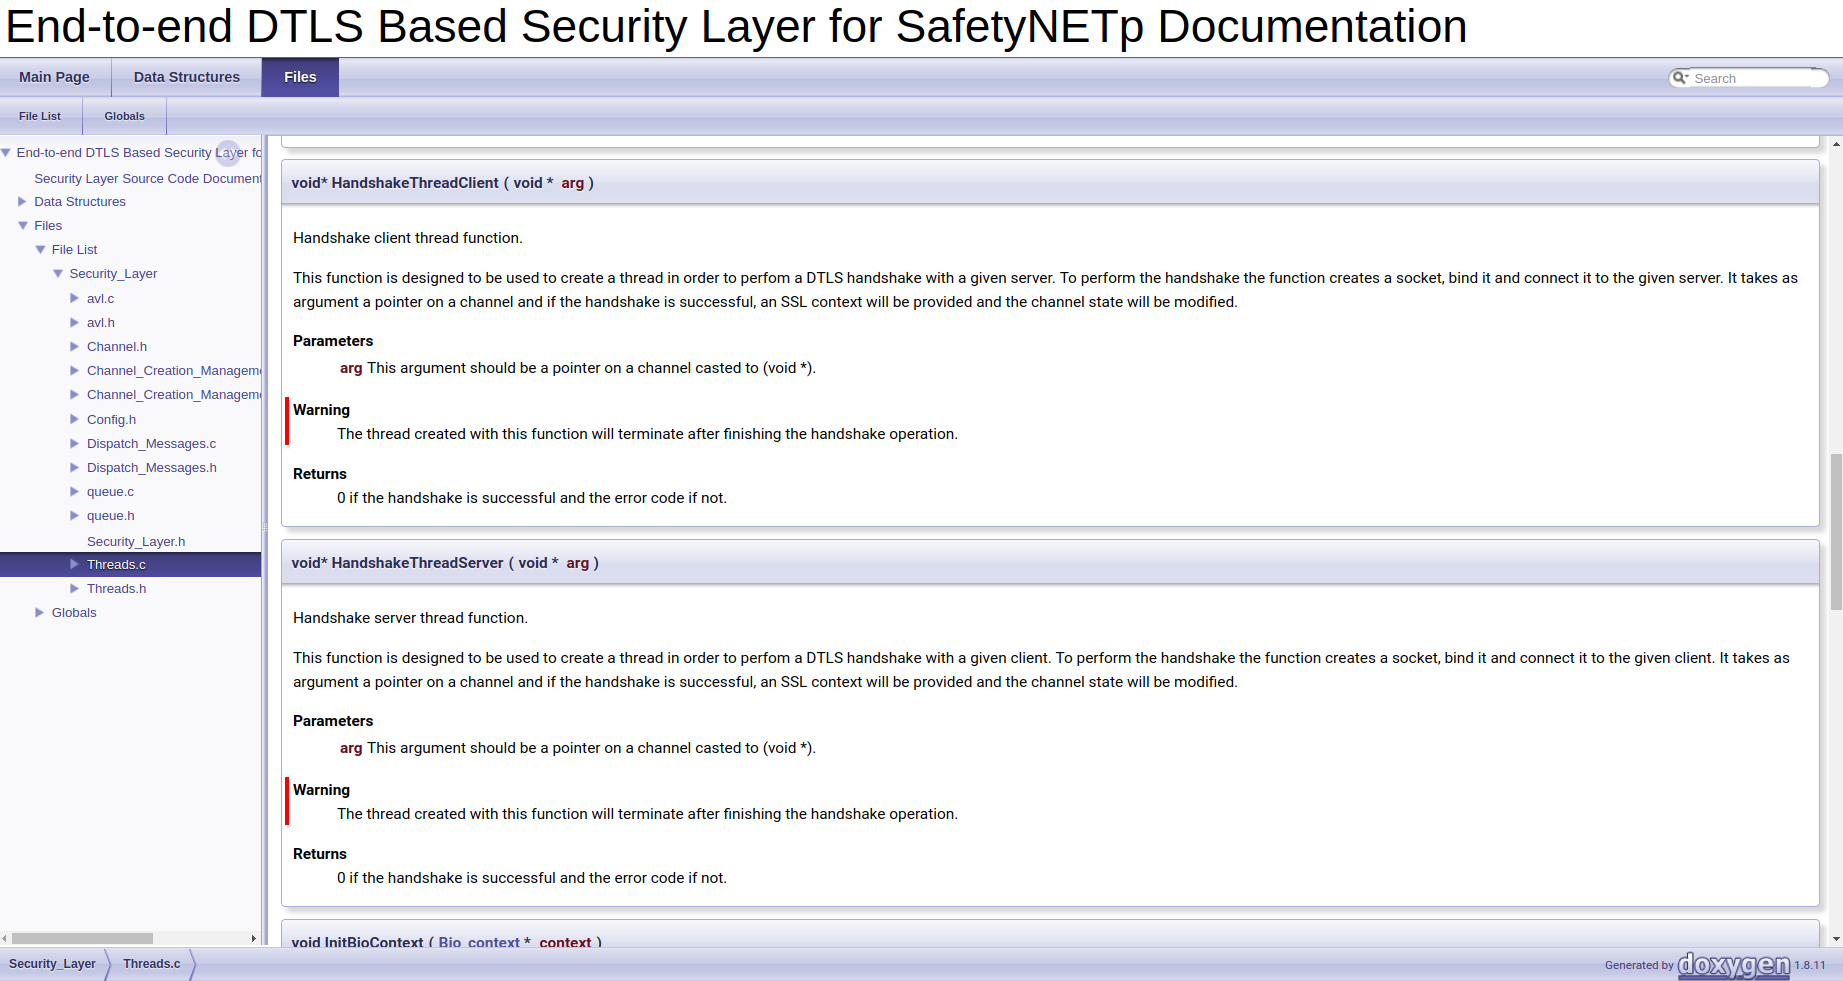
\includegraphics[width=19cm]{figures/realization/documentation_capture.png}
% \caption{Documentation capture}\label{documentation}
% \end{figure}


\subsection{Hardware Environment}

For the realization of this project, Pilz, the company which created SafetyNETp protocol, provided us with two Revolution Pis
containing their SafetyNETp implementation. The Revolution Pi (\autoref{revpi}) is a small computer designed by the Kunbus german company
based on the Rasberry Pi Compute Module. Unlike Rasberry Pi which is not designed for an industrial usage, the Revolution
Pi is designed to fit in industrial environments. As shown in \autoref{revpi_specs}, the Revolution Pi
has a protection against electrostatic discharge and electromagnetic interference according to the norms EN 61131-2 and IEC 61000-6-2.
In operating mode, the Revolution Pi could support a temperature between -40  $^\circ$C and +55 $^\circ$C which exceeds
the requirements of the norm EN 61131-2. The Revolution could be alimented by a power supply between 10.7 V and 28.8 V.
These characteristics make the Revolution Pi suitable for industrial usage \cite{revpi}.

\begin{table}[H]
    \begin{tabular}{|l|l|}
      \hline
      Processor & BCM2835, 700 MHz, single-core \\
      \hline
      RAM & 500 MByte \\
      \hline
      Electrostatic discharge protection & 4 kV / 8 kV (according to EN 61131-2 and IEC 61000-6-2) \\
      \hline
      Electromagnetic interference protection & Passed (according to EN 61131-2 and IEC 61000-6-2) \\
      \hline
      Surge/Burst tests & Passed (according to EN 61131-2 and IEC 61000-6-2) \\
      \hline
      Power supply &  min. 10.7 V - max. 28.8 V \\
      \hline
      Operating temperature & -40  $^\circ$C to +55 $^\circ$C(exceeds EN 61131-2 requirements) \\
      \hline
      Storage temperature & -40 $^\circ$C to +85 $^\circ$C (exceeds EN 61131-2 requirements) \\
      \hline
  \end{tabular}
  \caption[Revolution Pi characteristics]{Revolution Pi characteristics \cite{revpi}}
  \label{revpi_specs}
\end{table}

\begin{figure}[H]
\centering
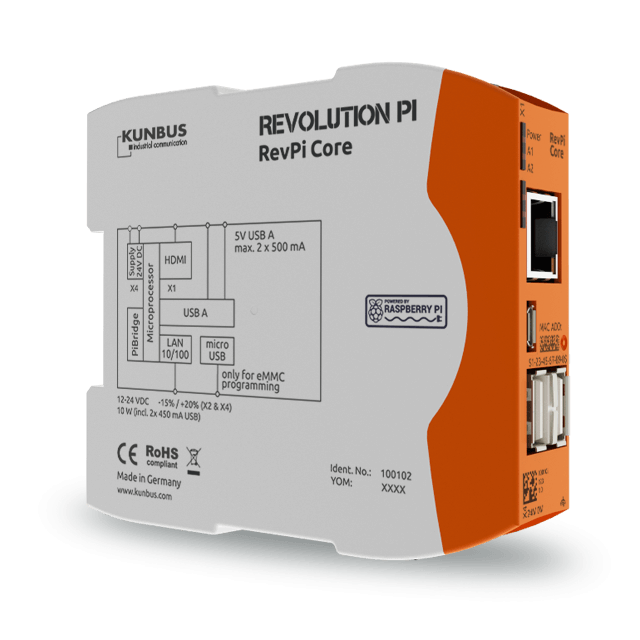
\includegraphics[width=9cm]{figures/realization/revpi.png}
\caption{Revolution Pi}\label{revpi}
\end{figure}

For the development, we used a laptop with the characteristics shown in \autoref{computer_characteristics}.

\begin{table}[H]
\centering
    \begin{tabular}{|l|l|}
      \hline
      Processor & Intel core i5 \\
      \hline
      RAM & 8 Gbyte \\
      \hline
      Graphics & Intel HD Graphics 620 \\
      \hline
  \end{tabular}
  \caption{Used computer characteristics}
  \label{computer_characteristics}
\end{table}

For interconnecting the Revolution Pis and our laptop we used a hub and Ethernet cables.

\section{Implementation}

In this section, we see the several steps we went through in order to implement our design.

\subsection{DTLS Implementation Choice}

Various DTLS implementations exists which support DTLS up to its final version, among these, we can cite:

\renewcommand{\labelitemi}{$\bullet$}
\begin{itemize}
\item \textbf{OpenSSL} \cite{OpenSSL}: This is an open source project that provides a robust, commercial-grade and
full-featured toolkit for SSL/TLS protocols. It is also a general-purpose cryptography library.
The OpenSSL toolkit is licensed under an Apache-style license, which basically means that
you are free to get and use it for commercial and non-commercial purposes subject to some
simple license conditions.

\item \textbf{WolfSSL} \cite{WolfSSL}: WolfSSL is a lightweight portable embedded SSL/TLS library written in ANSI C.
With its small size, speed, and feature set, WolfSSL targets embedded systems and resource-constrained environments.
It implements TLS and DTLS up to their latest versions which are currently TLS 1.2 and DTLS 1.2 and provides
progressive ciphers such as ChaCha20, Curve25519, NTRU, and Blake2b. This
software falls into the General Public License (GPL) and in case of commercial software
products, a commercial license must be bought.

\item \textbf{MatrixSSL} \cite{MatrixSSL}: MatrixSSL is an embedded SSL and TLS implementation designed for
small footprint IoT devices requiring low overhead per connection. The library is less than 50Kb on disk
with cipher suites. It includes client and server support through TLS 1.2, mutual authentication,
 and implementations of RSA, AES, SHA, SHA-256 and more.

\item \textbf{MbedTLS} \cite{MbedTLS}: formerly known as PolarSSL, it is an open source embedded SSL/TLS library provided by arm and written in C.
Its small memory footprint makes it suitable for embedded environments. MbedTLS provides an up to date implementations of both TLS and DTLS.
MbedTLS is primarily licensed under the Apache 2.0 license and a packaged version is available under the GPL as well.
Therefore MbedTLS could be used for free for both commercial and non-commercial use.
\end{itemize}

In fact, we decide to use MbedTLS for the following reasons \cite{MbedTLS}:

\renewcommand{\labelitemi}{$\bullet$}
\begin{itemize}
\item \textbf{Tiny and portable library}: As MbedTLS is written in C, it is portable and suitable for embedded environments.
\item \textbf{Easy to understand and use with a clean API}: MbedTLS offers a readable code and a logical,
clean, and well-documentated API. MbedTLS provides a reference and a high-level design for its API (using UML diagrams) making
understanding and using the library a lot easier.
\item \textbf{Easy to reduce and expand the code}: MbedTLS has no global code and has minimal coupling between its modules.
So it's easy to just grab a part and drop it into an existing project or add new functionality.
\item \textbf{Apache and GPL licenses}: MbedTLS could be used for free in open source and non-open source project
as well as in commercial and non-commercial projects.
\end{itemize}

\subsection{SafetyNETp Plugin Implementation for Wireshark}

To be able to understand the behavior of SafetyNETp devices, the first step was to analyze
the traffic exchanged between the two devices provided by Pilz. For this purpose, we used
the well-known traffic analyzer Wireshark. As SafetyNETp is proprietary protocol, it is difficult
to find information about its functioning or its packet format in public sources. In fact, Wireshark
does not recognize SafetyNETp packets, hence, the messages are shown as raw data. Analyzing raw data messages
makes our task extremely difficult. \autoref{safetynetp_raw_messages} shows a Wireshark capture of a data exchange between two
SafetyNETp devices. As the figure shows, no message type is mentioned, Wireshark just presents SafetyNETp's data
as UDP payload.


\begin{figure}[H]
\centering
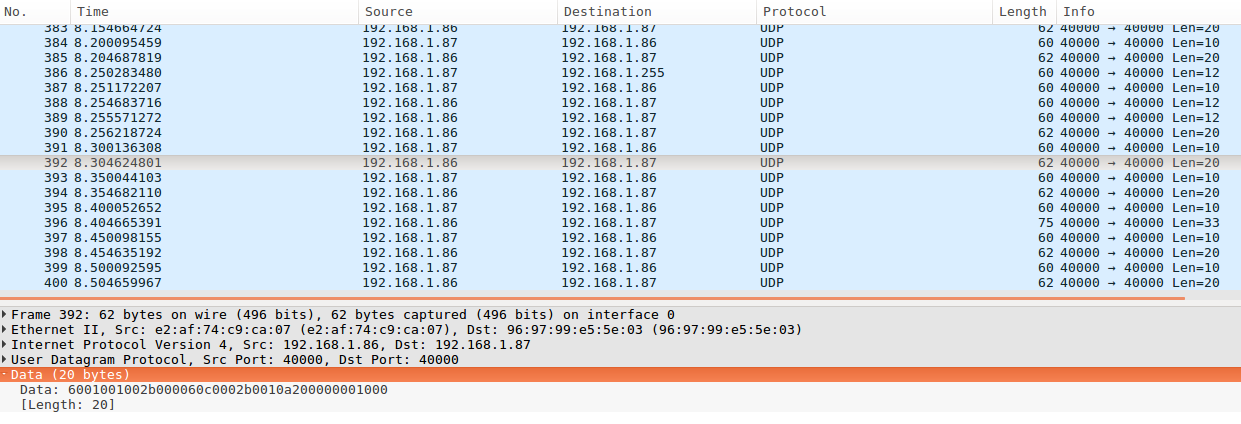
\includegraphics[width=17cm]{figures/realization/safetynetp_raw_messages.png}
\caption{Wireshark capture without our plugin}\label{safetynetp_raw_messages}
\end{figure}

To facilitate analyzing and debugging the exchanged messages, we implemented a Wireshark plugin using lua
programming language which enables the support of SafetyNETp in Wireshark. The \autoref{safety_plugin} shows a
capture after we have integrated our plugin into Wireshark. The exchanged messages are no longer shown as raw
UDP payload, instead, our plugin takes the responsibility for interpreting SafetyNETp packets and shows
their types. Furthermore, we are able to use filters, allowing for example to see only specific messages types.

\begin{figure}[H]
\centering
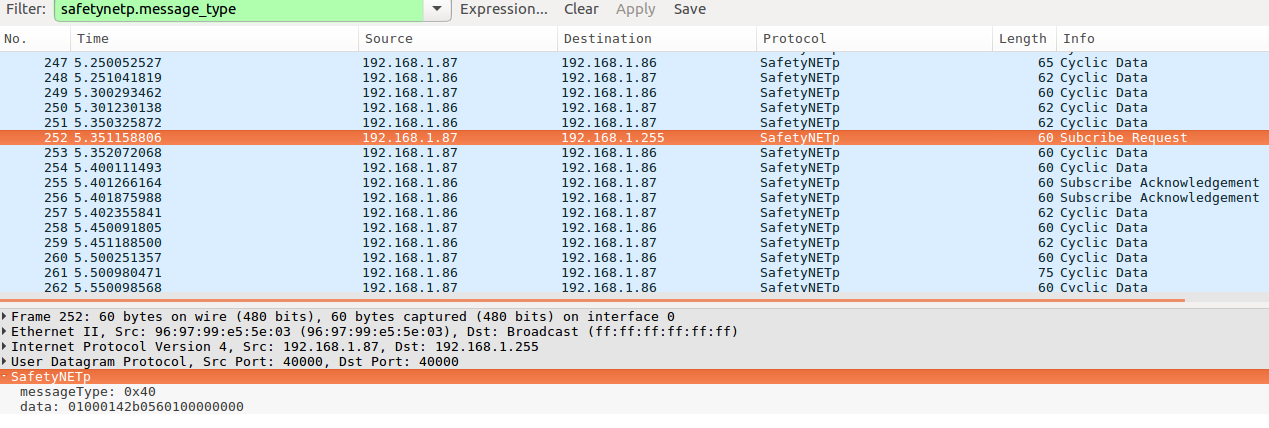
\includegraphics[width=17cm]{figures/realization/safety_plugin.png}
\caption{Wireshark capture after integrating our plugin}\label{safety_plugin}
\end{figure}

\subsection{Threads and Socket Managment}

As the Revolution Pis run Linux Debian, for exchanging data over the network,
SafetyNETp uses the Linux socket API. In fact, a socket is an abstraction through which an application
may send and receive data, in much the same way as an open file allows an application to read and write data.
A socket allows applications to communicate over the network, an information written to a socket
by an application on one machine can be read by an application on a different machine and
vice versa. Numerous types of sockets exist, for our case, we will be using UDP sockets.

Every SafetyNETp device using our security layer implementation runs several threads.
As shown in \autoref{sockets}, four kinds of threads are present:

\renewcommand{\labelitemi}{$\bullet$}
\begin{itemize}
\item \textbf{The first handshake thread}: This could be a client or a server thread, its role is to establish
the first handshake. This thread terminates when the handshake finishes.

\item \textbf{The receiving data thread}: This thread is responsible for receiving, decrypting, and verifying
data. The thread terminates when its session is closed.

\item \textbf{Session renewal thread}: This could be a client or a server thread, its role is to
establish a new handshake in order to renew the keying material. This thread terminates when the handshake
finishes or its session is closed.

\item \textbf{Sending data thread}: This thread is responsible for sending both protected and unprotected
data. This thread runs while the device is on.
\end{itemize}

In each device, one single thread exists for sending data, and $n$ threads exist for receiving data, with $n$
the number of channels. In fact for each connection, a \textit{first handshake thread} is created for establishing
the first handshake, then a \textit{receiving data thread} is created for receiving, decrypting, and verifying
data, furthermore, periodically, a \textit{session renewal thread} is created to renew the keying material.

For sending and receiving data, we have two possibilities, whether we create one single socket for all devices, or
create and dedicate a specific socket for each device. A socket has separate buffers for writing and reading
which means that it is possible to have two threads, one writing and one reading at the same time. However, having two
threads writing to a socket at the same time is not possible. We could have the case where a device is for example
establishing multiple handshakes with $n$ devices at the same. In this case, $n$ handshake threads will be running at the same
time. If we use one single socket, we need to manage the threads access for writing into the socket as it is not
possible to perform more than one write operation at the same time. Furthermore, when receiving a packet,
our application has to filter the incoming packets to know their sources as all the devices send their data
on the same socket. That's why, as shown in \autoref{sockets}, a separate socket is created for each device. Hence, having multiple
handshake threads does not cause access problem anymore as each thread will be writing on a separate socket. In
addition, no filtering is needed, the linux kernel will filter the packets according to the sockets.

\begin{figure}[H]
\centering
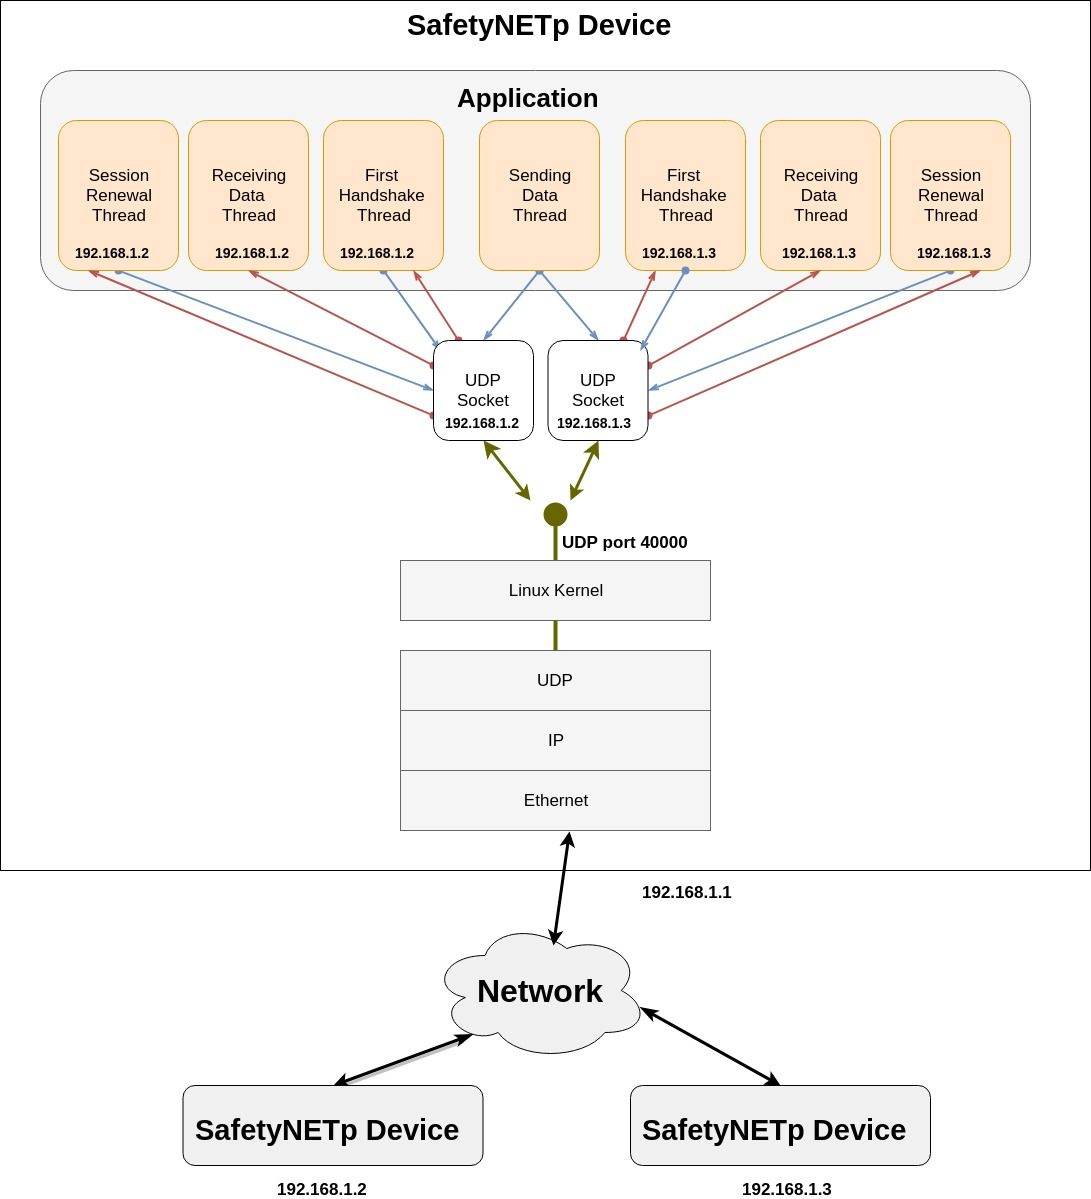
\includegraphics[width=13cm]{figures/realization/sockets.jpg}
\caption{Threads and sockets}\label{sockets}
\end{figure}

As mentioned in the previous chapter, we need to renew periodically the keying material to minimize cryptanalysis
attacks. This corresponds in our implementation to create a \textit{session renewal thread}. It is obvious that the \textit{session renewal thread} needs to write and read data from the dedicated socket. Meanwhile, the \textit{sending data thread} is
sending cyclically \textit{cyclic data} which means that it is writing to the socket. Therefore, we could end up
having simultaneous access to the socket. We can manage the simultaneous access by using a mutex variable to
protect writing on the socket, in fact, this solves the problem by letting only one thread writing at a time.
\autoref{mutex_write_socket} shows how the socket concurrent access is managed. If we assume that the green state is the
current, in this case, the \textit{sending data thread} will wait until the \textit{session renewal thread} writes and unlocks
the socket. Such management could delay sending \textit{cyclic data} that's why we need to avoid this method.

\begin{figure}[H]
\centering
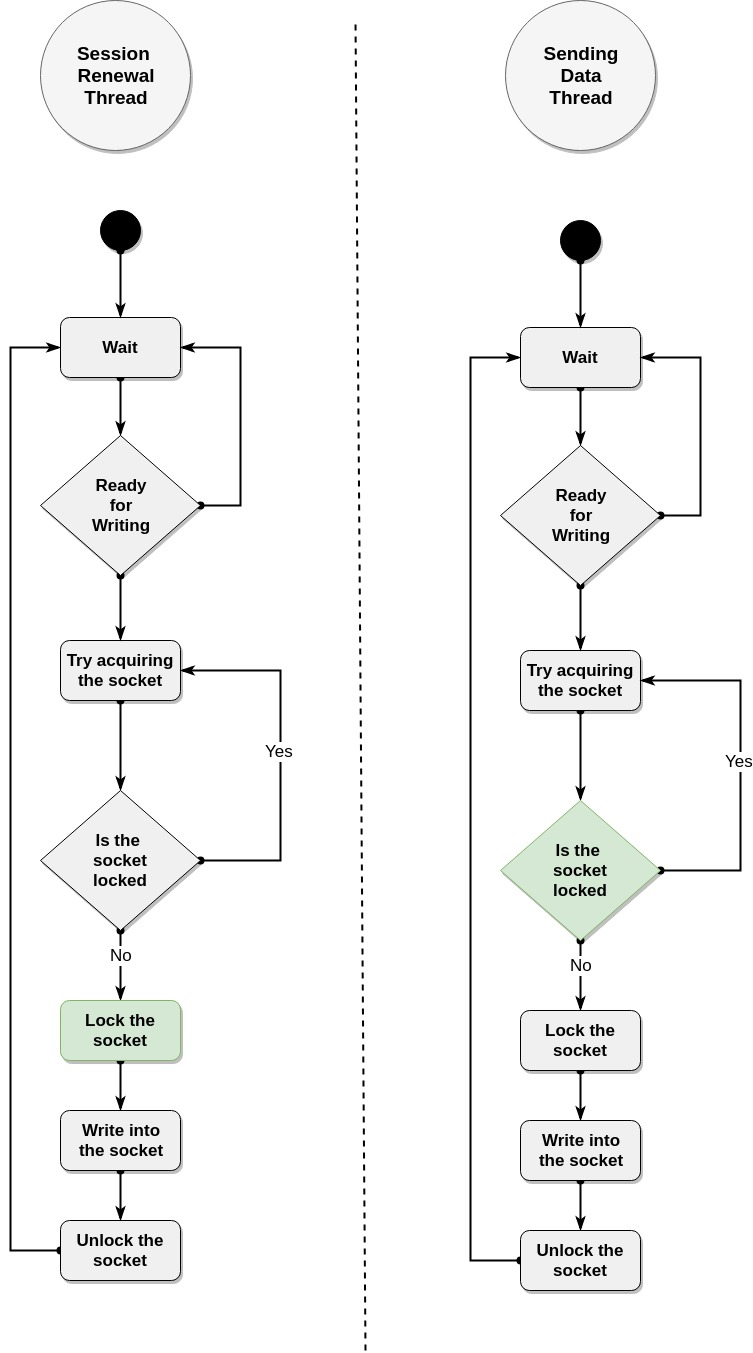
\includegraphics[width=10cm]{figures/realization/write_to_queue.jpg}
\caption{Socket concurrent access}\label{mutex_write_socket}
\end{figure}

To avoid delaying \textit{cyclic data}, we will not allow the \textit{session renewal thread} to access the socket directly.
Instead, it writes the message on a queue and only the \textit{sending data thread} will have access to the sockets.
When the \textit{sending data thread} sends a message, it verifies the queue which contains the messages written by the
\textit{session renewal thread}. If the queue is not empty, the \textit{sending data thread} dequeues the first message and sends it.
Using this method, we ensure that the \textit{cyclic data} is sent immediately without any additional delay (\autoref{write_to_queue}).

\begin{figure}[H]
\centering
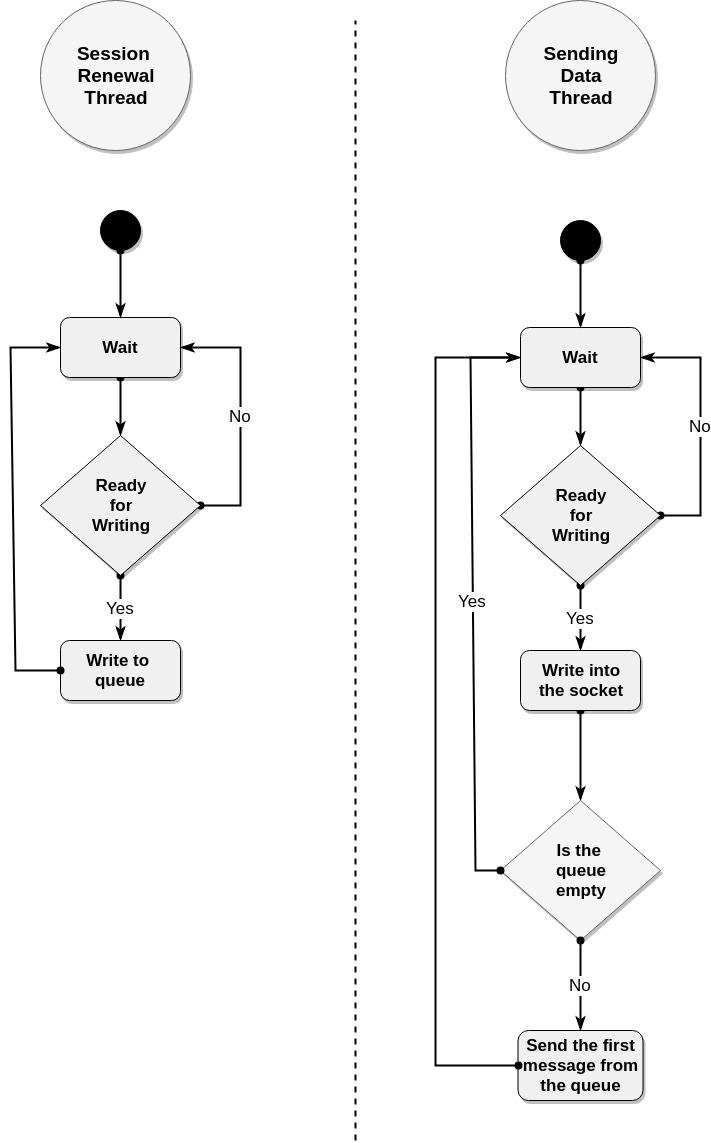
\includegraphics[width=8cm]{figures/realization/mutex_write_socket.jpg}
\caption{Prioritization of \textit{cyclic data} messages over handshake messages}\label{write_to_queue}
\end{figure}

\subsection{Channel Lookup}

Each SafetyNETp device can obviously communicate with multiple other devices. For instance, a publisher could
be publishing data for an arbitrary number of $n$ subscribers. The publisher will have a list of secure channels, each one is used
to communicate securely with one subscriber. Each channel has as an identifier the IP address of the subscriber.
For each \textit{cyclic data} message to be sent, the publisher has to fetch the list of channels and to find
the corresponding channel to use for the destination devices. Having a big number of channels
could affect the cycle time that’s why we will be interested in this section in selecting a search
algorithm that allows keeping the cycle time as it is as much as possible.

In order to find the channel to use, we need to find the one which has the corresponding IP address which is no
more than a 4 bytes integer. As a result, the problem is about finding an integer in a given list.
The classic method for searching is linear search, given a list of $n$ elements, it sequentially checks
each element of the list for the target value until a match is found or until all the elements have been
searched. the complexity of the linear search method is equal to $O(n)$.

% \begin{figure}[!htbp]
% \centering
% 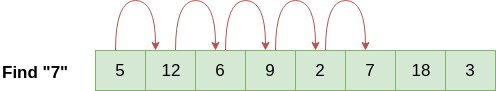
\includegraphics[height=2cm]{figures/design/linear_search.jpg}
% \caption{Linear search}\label{linear_search}
% \end{figure}

Another method is commonly used which is the binary search tree, it searches in a sorted list by
repeatedly dividing the search interval in half. Begin with an interval covering the whole list. If the
value of the search key is less than the item in the middle of the interval, narrow the interval to the
lower half. Otherwise, narrow it to the upper half. Repeatedly check until the value is found or the
interval is empty. The complexity of the binary search method is $O(log(n))$ if the tree is balanced, however,
if it is unbalanced it could reach a complexity of $O(n)$.

% \begin{figure}[H]
% \centering
% 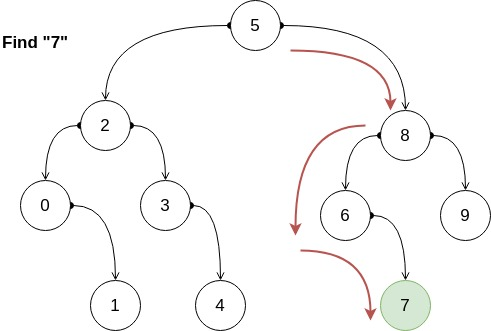
\includegraphics[height=7cm]{figures/design/binary_search_tree.jpg}
% \caption{Binary search tree}\label{binary_search_tree}
% \end{figure}

To get rid of the balancing problem, AVL is the solution. AVL tree is a self-balancing binary
search tree where the difference between heights of left and right subtrees cannot be more than one
for all nodes. Most of the binary search tree operations (search, max, min, insert, delete, etc) take
$O(h)$ time where $h$ is the height of the binary search tree. The cost of these operations may become
$O(n)$ for a skewed Binary tree where $n$ is the number of nodes. If we make sure that height of the tree remains $O(log(n))$ after every
insertion and deletion, then we can guarantee an upper bound of $O(log(n))$ for all these operations.
The height of an AVL tree is always $O(log(n))$ where $n$ is the number of nodes in the tree.

\begin{figure}[H]
\centering
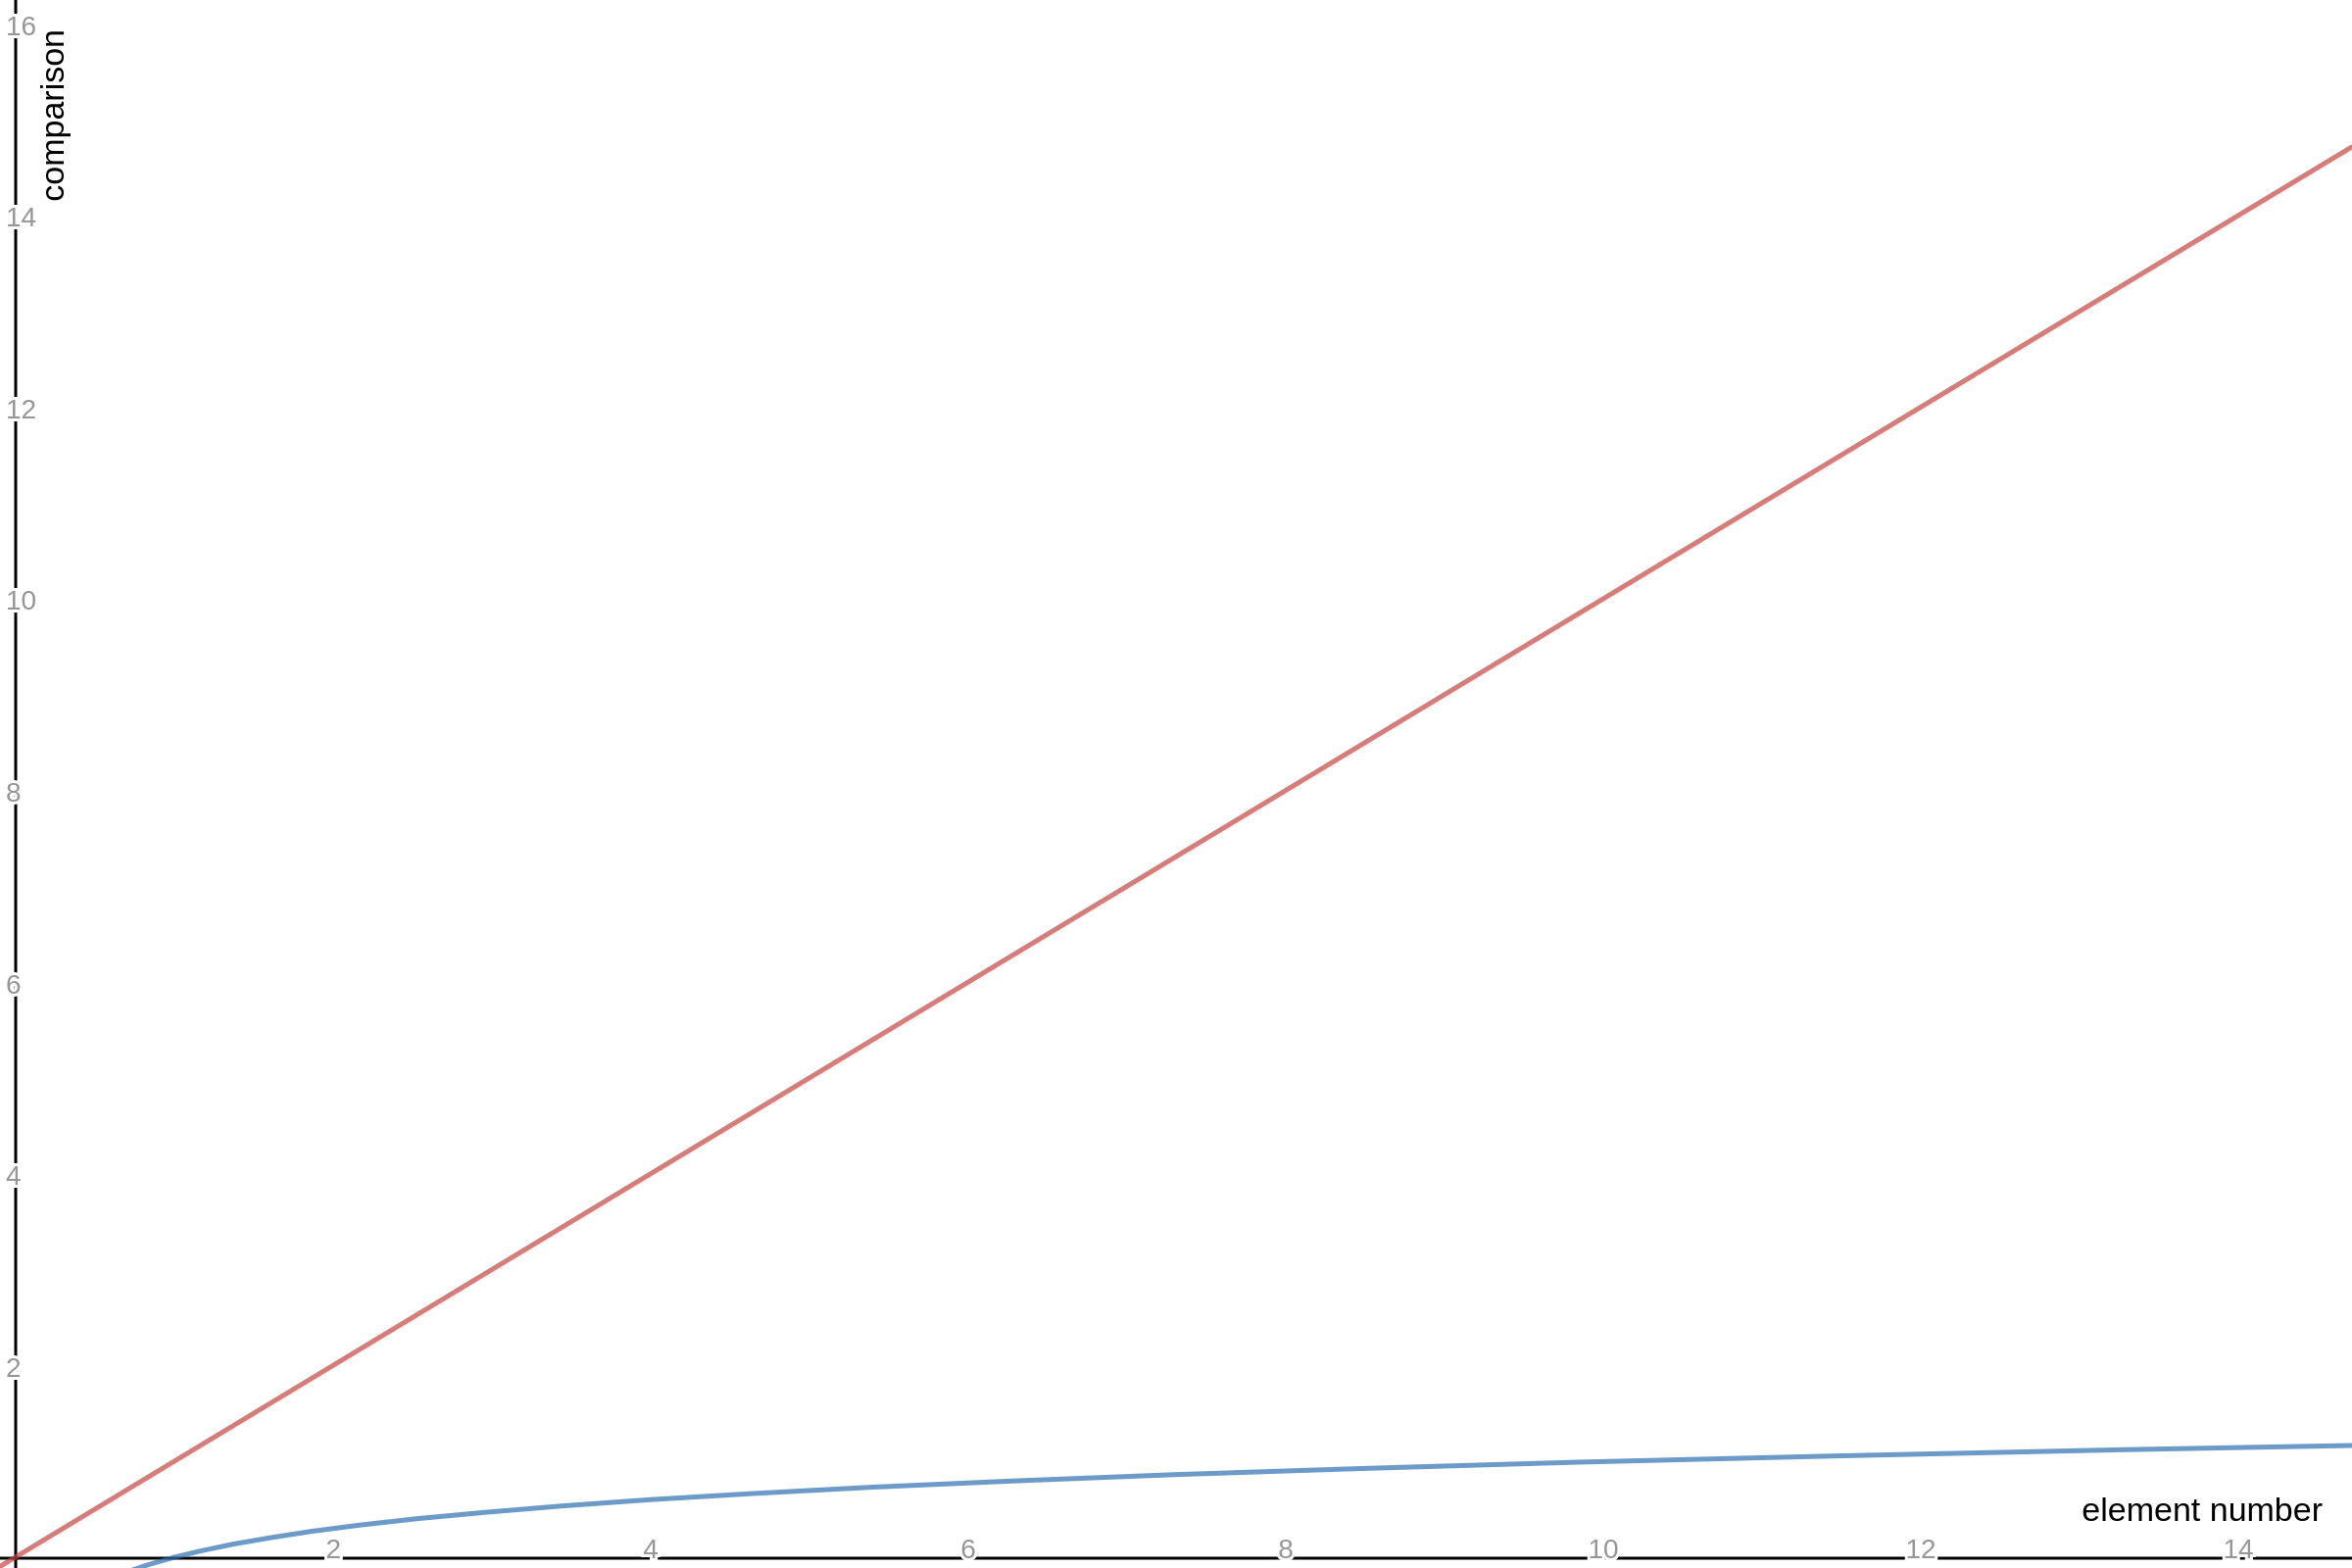
\includegraphics[height=7cm]{figures/design/comparison_between_search_methods.png}
\caption{Comparison between $O(n)$ and $O(log(n))$}\label{comparison_between_search_methods}
\end{figure}

\autoref{comparison_between_search_methods} shows the two functions $n$ in red and $log(n)$ in blue it shows in
other words how increasing the number of elements will affect the number of comparisons to be performed in order
to find the target. It is clear that $log(n)$ is always below $n$ which means that the number
of comparisons is always smaller. As a result, we used the binary search tree method.

\section{Implementation Demo and Performance Test}

As shown in \autoref{test_environment}, our test environment consists of two Revolution Pis, a power supply and
a hub for interconnecting the Revolution Pis with our laptop.
The Revolution Pis are configured to subscribe mutually to each other, they have 192.168.1.86
and 192.168.1.87 as IP addresses.
In this section we go into an overview to see the implementation demo, then we move to the test.

\begin{figure}[H]
\centering
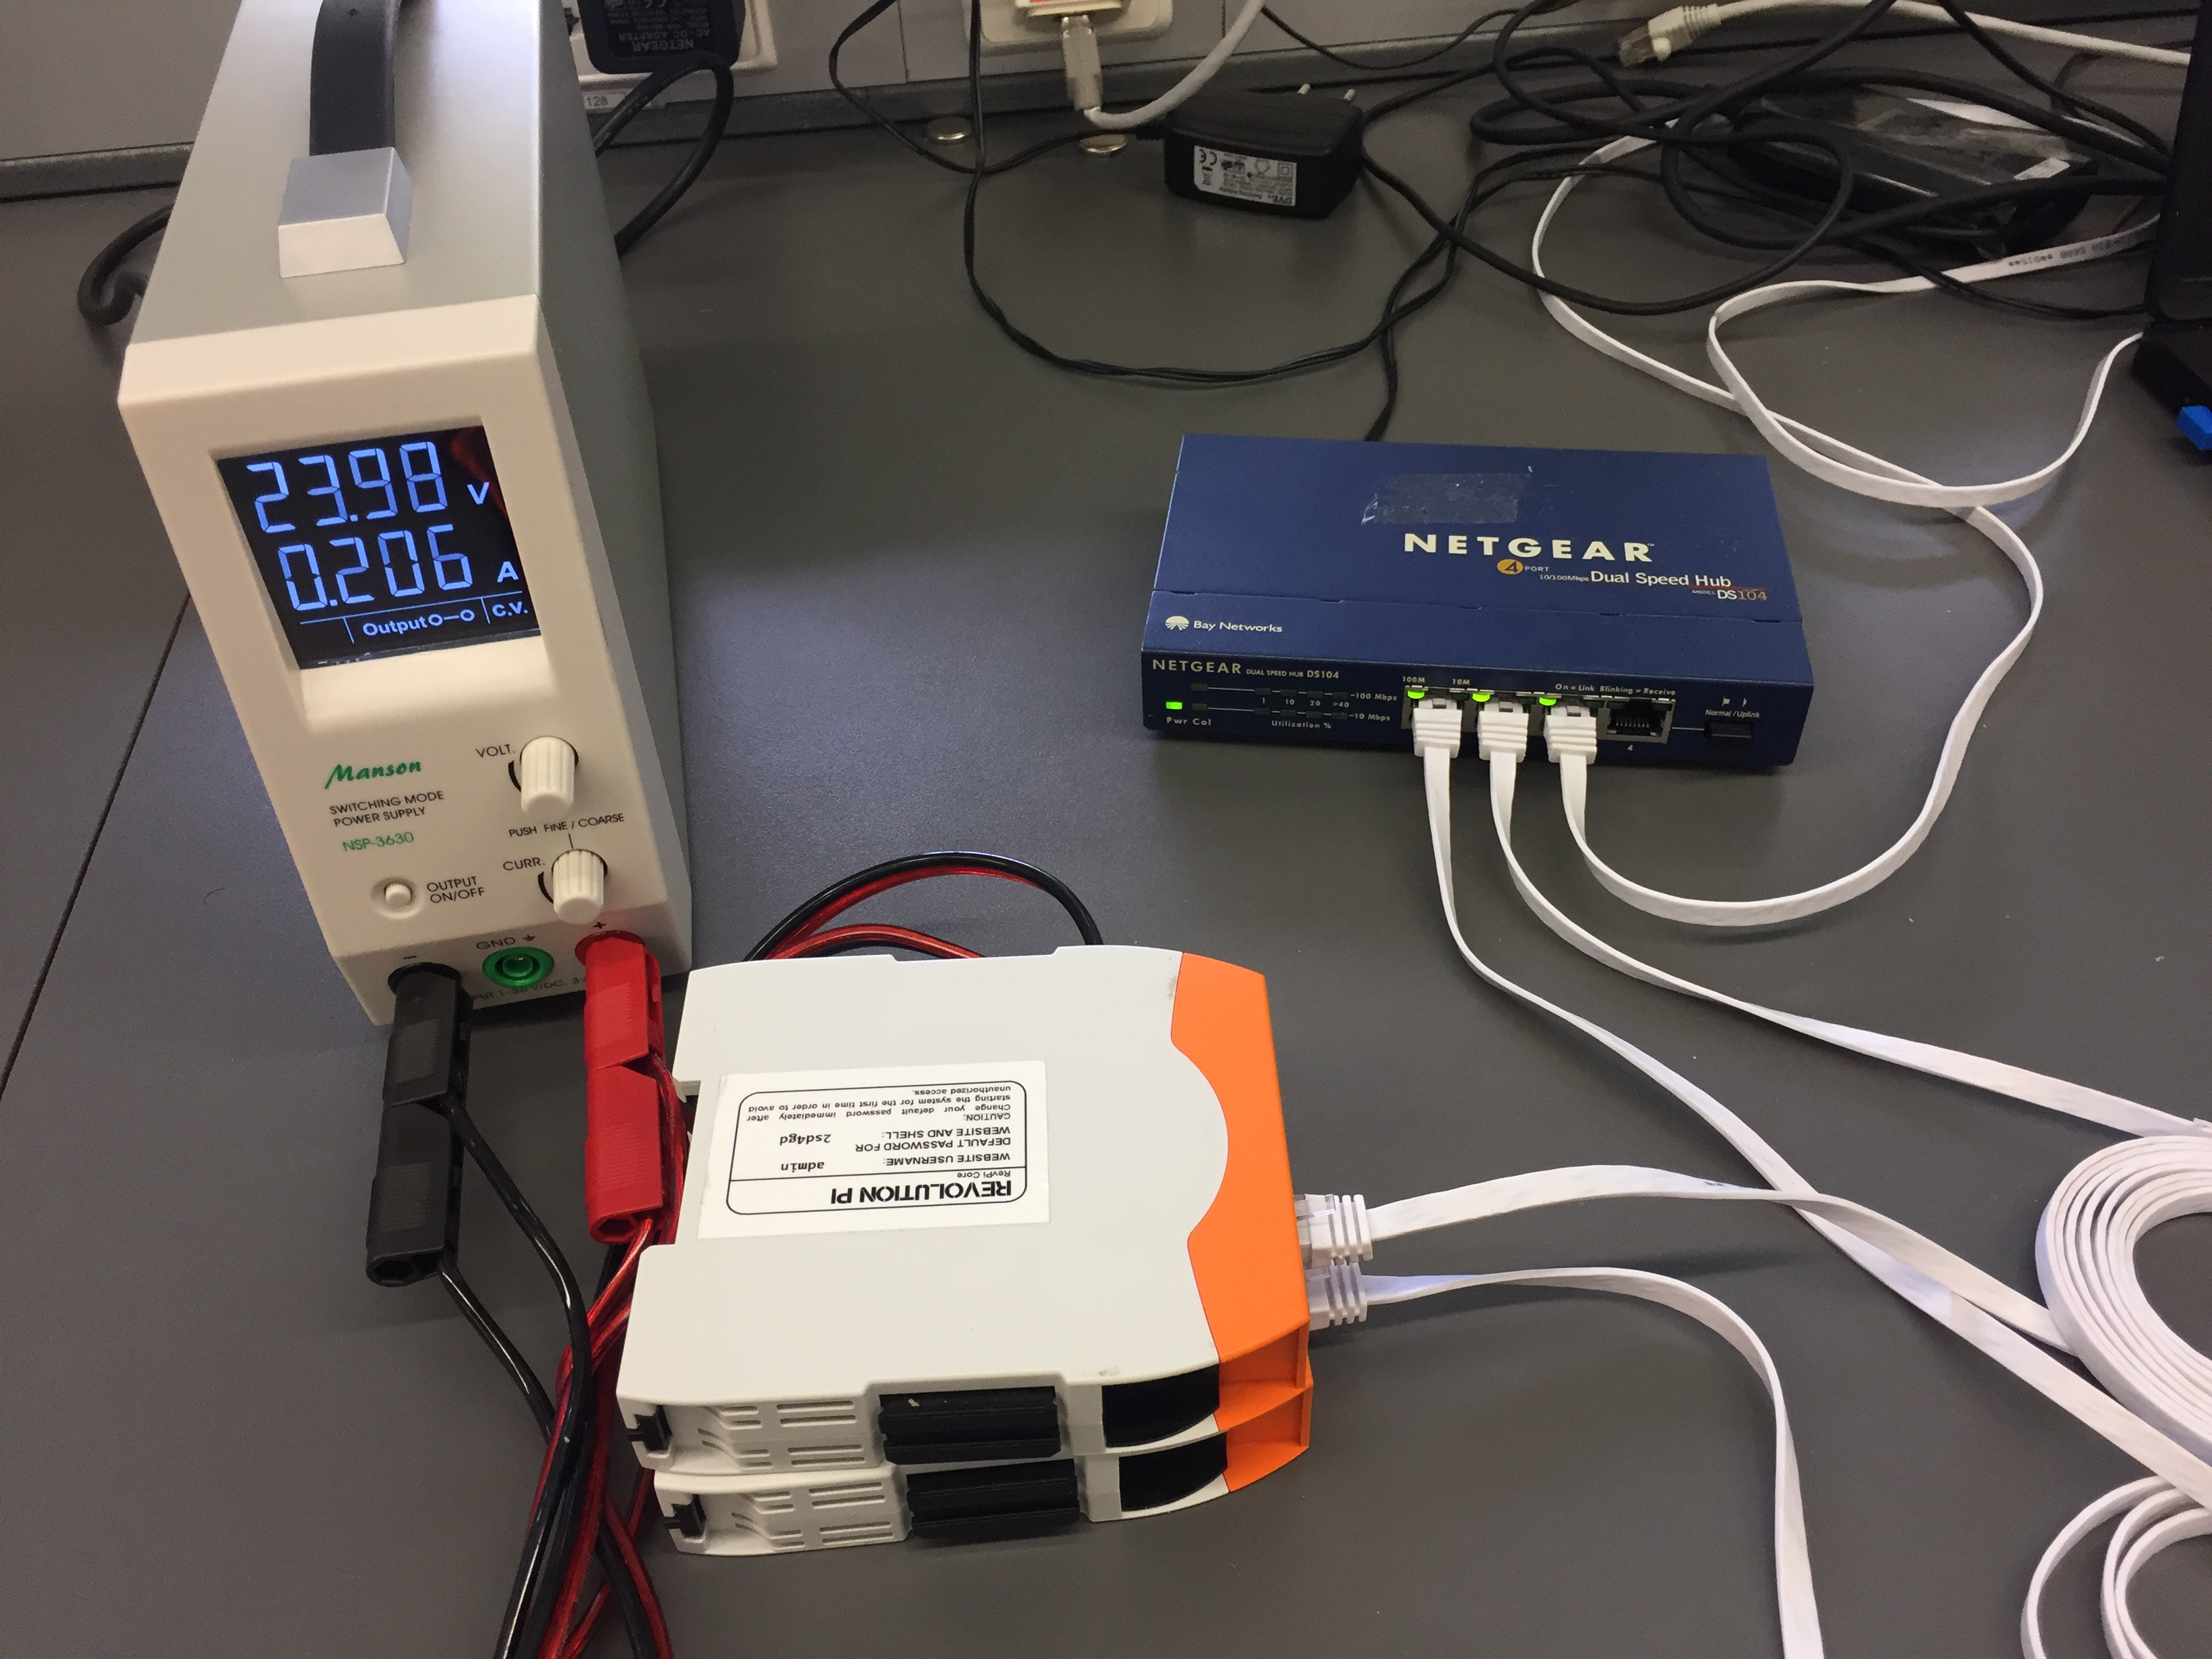
\includegraphics[width=10cm,height=6cm,frame]{figures/realization/test_environment.JPG}
\caption{Test environment}\label{test_environment}
\end{figure}

\subsection{Demo}

The \autoref{first_handshake} shows the case where the communication is initiated and the first handshake is established.
In fact, as we mentioned in the design chapter, the DTLS roles are chosen based on the IP addresses.
The right capture is the screen of the device which has the IP address 192.168.1.87 and left one
corresponds to the device which has the IP 192.168.1.86. As we can see the device with the higher IP launched
a server thread whereas the device with the smaller IP launched a client thread. After launching the threads,
they begin establishing the handshake and they exchange their certificates. Thereafter, each end-point
verifies the other end-point's certificate. As we see in this capture, the certificates are verified correctly and
therefore they start exchanging secured \textit{cyclic data}.

\begin{figure}[H]
\centering
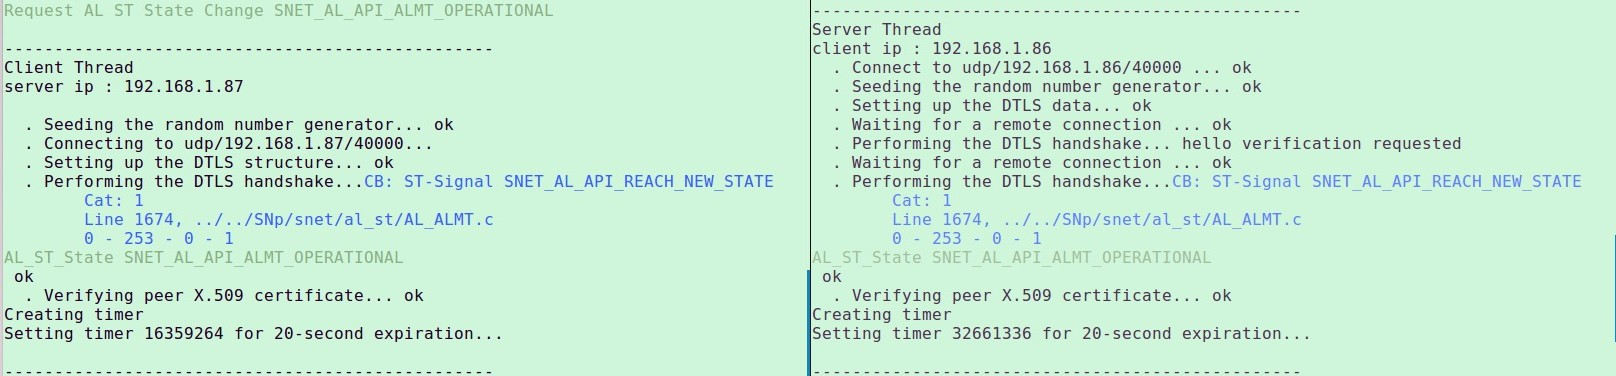
\includegraphics[width=19cm,frame]{figures/realization/first_handshake(1).jpg}
\caption{The first handshake establishment}\label{first_handshake}
\end{figure}

In order to minimize the risk of cryptanalysis attacks, as mentioned in the previous chapter,
a new handshake is run each a well defined period of time. For test purposes, we set the period of session renewal
to 20 seconds. As shown in \autoref{session_renewal_threads}, each 20 seconds the devices launch a \textit{renewal session thread}
in order to establish a new handshake. Following each established handshake, the \textit{channel id} header
field is incremented to allow the receiving devices to verify and decrypt the messages with right keying
material.

\begin{figure}[H]
\centering
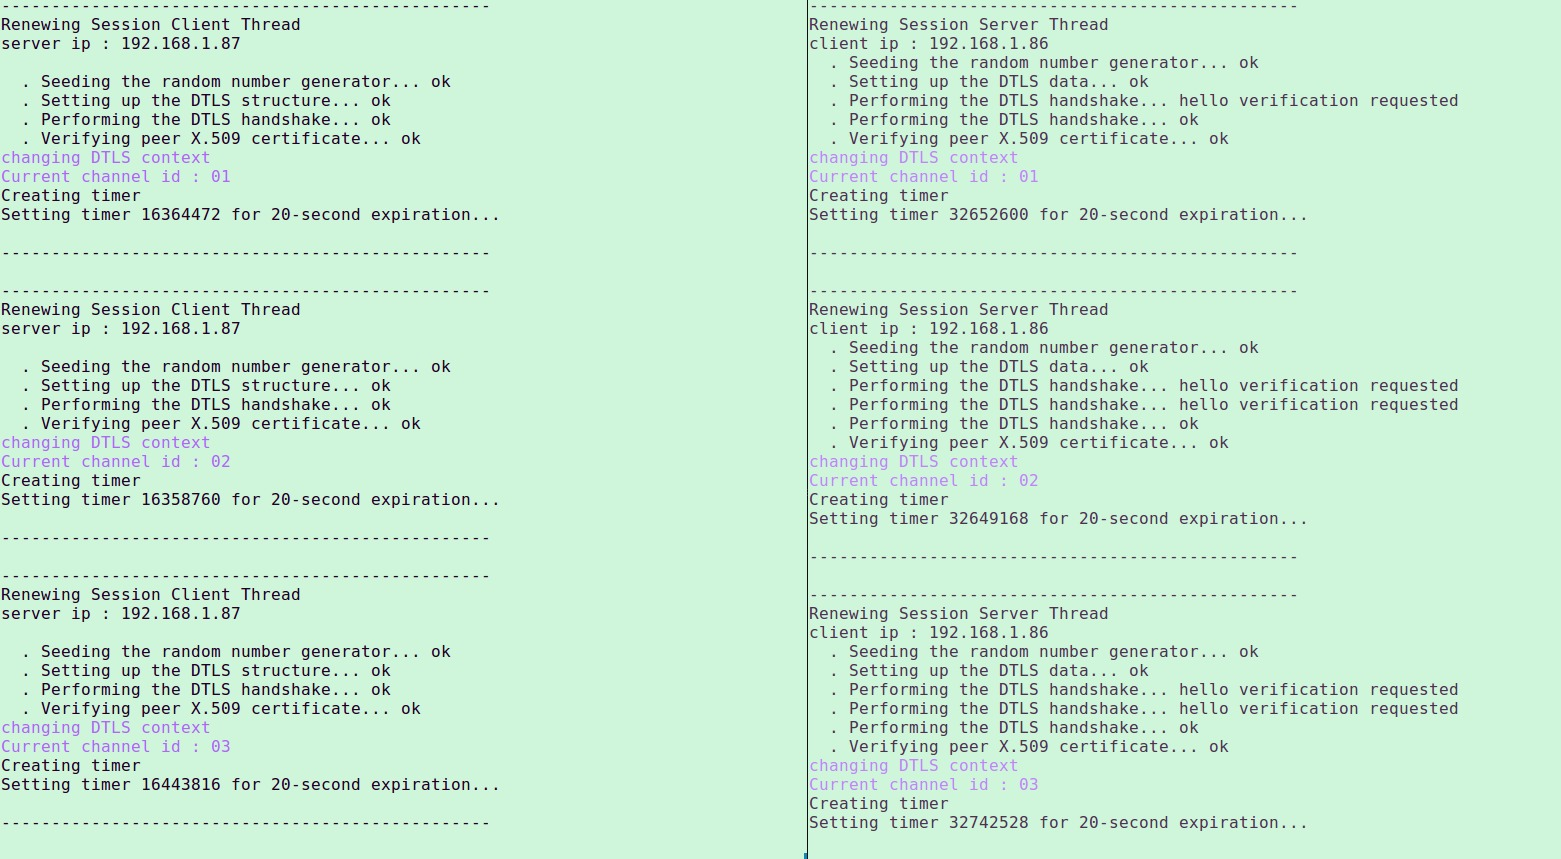
\includegraphics[width=19cm,frame]{figures/realization/session_renewal(2).png}
\caption{Session renewal threads}\label{session_renewal_threads}
\end{figure}

The main difference between the \textit{first handshake thread} and the \textit{renewal session thread} is
that while establishing the first handshake the cyclic data is blocked as the identity of
the second end-point could not be verified before
finishing the handshake. However, when renewing the keying material, the cyclic data is sent,
and the new handshake's messages should be sent without interrupting sending cyclic data.
The \autoref{cyclic_data_time_out} shows the message which SafetyNETp application layer logs when
the timeout of the cyclic data expires. As shown in \autoref{session_renewal_threads} no such message
is logged which confirms that the handshakes are being established without interrupting sending the cyclic data.

\begin{figure}[H]
\centering
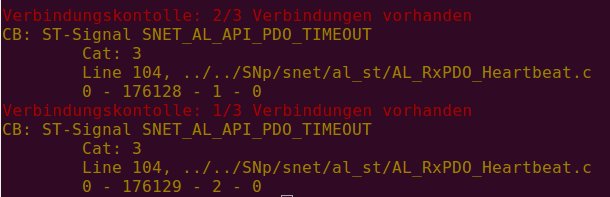
\includegraphics[width=10cm]{figures/realization/cyclic_data_time_out.png}
\caption{SafetyNETp timeout log}\label{cyclic_data_time_out}
\end{figure}

The \autoref{safetynetp_original_message} shows a Wireshark capture of a cyclic data message sent unprotected as plaintext
before integrating our security
layer. The \autoref{secured_cyclic_data_message} shows a Wireshark capture of a cyclic data message sent through our security layer.
The first byte of the secured message is the security layer frame byte which is, in this case, \textit{0x88},
we chose arbitrarily this value and it could be changed via a configuration file. The second byte is the channel id
and the rest of the message is the SafetyNETp cyclic data message encapsulated into a DTLS frame.
We remark that the secured message is longer than the original message which is obvious as
additional data are included for encryption and for integrity checks.

\begin{figure}[H]
\centering
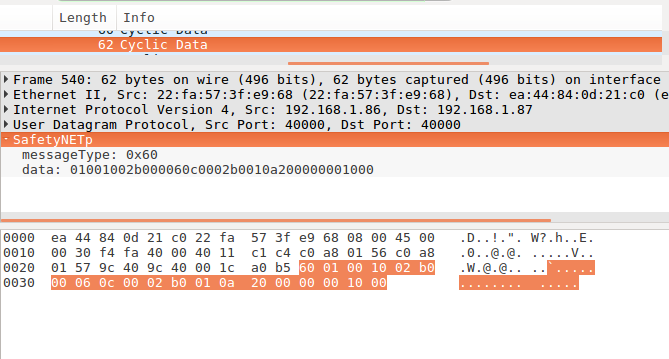
\includegraphics[width=12cm,frame]{figures/realization/unprotected_cyclic_data.png}
\caption{SafetyNETp original cyclic data message}\label{safetynetp_original_message}
\end{figure}

\begin{figure}[H]
\centering
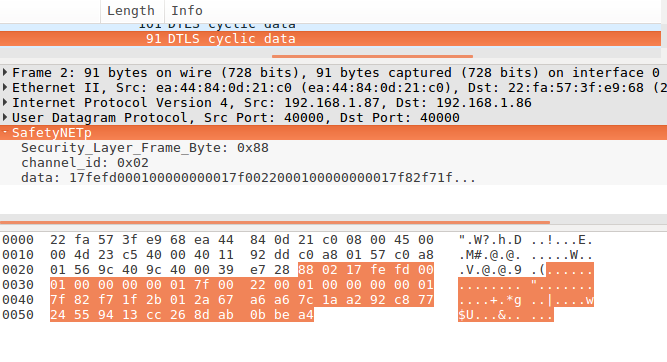
\includegraphics[width=12cm,frame]{figures/realization/secured_cyclic_data.png}
\caption{Secured cyclic data message}\label{secured_cyclic_data_message}
\end{figure}

In our security layer, when performing the DTLS handshake the devices' identities are verified using the certificate mechanism.
Therefore we have created our own \ac{PKI} in order to issue the devices' certificates. Our public key infrastructure
is composed from two \ac{CA}s, a root \ac{CA} and an intermediate \ac{CA}. The first step was to create the root CA by
generating its public and private keys and generating its certificate. In fact, the root CA's certificate is self-signed as it is
the first created CA. The second step was to create the intermediate CA, like creating the root CA, we generated the
public and the private keys as well as the certificate. However, the intermediate CA's certificate is not self-signed, it is actually
signed by the root CA. One could ask why do we need an intermediate CA when only the root CA is sufficient? In fact, it is a best practice to create an intermediate CA. The intermediate CA is used to issue and sign certificates on behalf of
the root CA. This minimizes the risks of compromising the root CA's private key.
After the creating the CAs, we issued a certificate for each device, thereafter, we configured the devices and added the root CA among the list of trusted CAs.
Creating the CAs as well as issuing the certificates is performed using three bash scripts that we have developed.
\autoref{cert_example} shows a certificate example which is, in this case, the intermediate CA's certificate.

\begin{figure}[H]
\centering
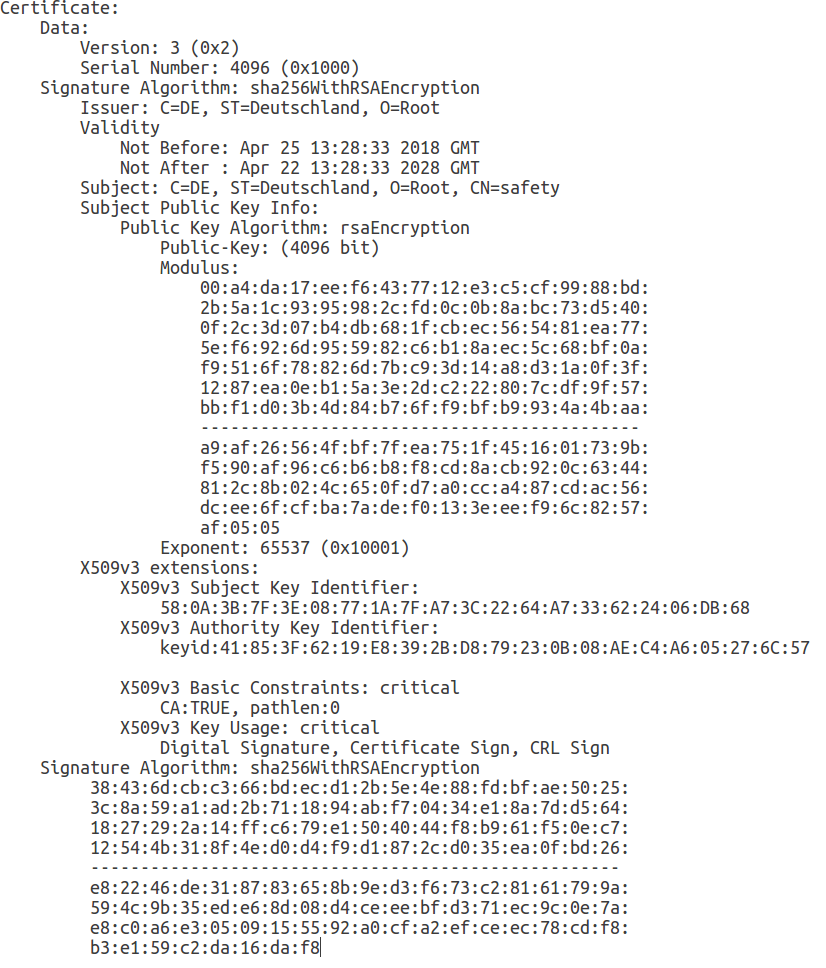
\includegraphics[width=12cm,frame]{figures/realization/certificate_example.png}
\caption{Certificate example}\label{cert_example}
\end{figure}

In order to facilitate modifying the parameters of the security layer, we created the configuration file
shown in \autoref{config_file}. Through this configuration file, SafetyNETp developers could easily change the security layer frame
byte, set the interval for renewing the keying material, set the max channel id value, print the sent and the received messages and print threads log to facilitate
debugging.

\newpage

%-------------------------------------------------------------------------------
%
%       Filename:  listing_two.tex
%
%    Description:  The file shows a hack for the use of lstlisting package with
%                  IfLanguagepackage
%
%        Version:  0.1
%        Created:  02.05.2016
%       Revision:  none
%
%         Author:  M.Sc. Oliver Kehret, oliver.kehret@hs-offenburg.de
%   Organization:  ivESK, Offenburg University, Germany
%      Copyright:  Copyright (c) 2016, M.Sc. Oliver Kehret
%
%-------------------------------------------------------------------------------
\begin{lstlisting}[caption={Security layer configuration file},label={config_file}]
/**
 * @brief Set Security Layer Frame byte value
 */
#define SECURITY_LAYER_FRAME_BYTE             0x88
/**
 * @brief Configure the renewing session interval in seconds
 */
#define RENEWING_SESSION_INTERVAL              20
/**
 * @brief Configure the period of time to wait after renewing the session to
 * switch using the new DTLS context
 */
#define DTLS_CONTEXT_SWITCH_TIME               4
/**
 * @brief Set the max value for the channel ID, when this value is reached
 * the next value will be 0x00
 */
#define MAX_CHANNEL_ID_VALUE                   0xff
/**
 * @brief Define this macro to print the Handshakes log
 */
#define PRINT_HANDSHAKE_LOG
/**
 * @brief Define this macro to print the Threads log
 * (Server and Client IP, channel ID, renewing session timer)
 */
#define PRINT_THREADS_LOG
/**
 * @brief Define this macro to print the outgoing messages (plaintext)
 */
#define PRINT_O_MSG
/**
 * @brief Define this macro to print the incoming messages (plaintext)
 */
#define PRINT_I_MSG
\end{lstlisting}




\subsection{Performance Test}

In this section, we present the results of the performed tests which consist of evaluating SafetyNETp with and
without the security layer. For this purpose, we have generated random messages with different lengths and we have calculated the time needed for sending and receiving them. In order to have more accuracy,
we have calculated the send and the receive time  1000 times for each length. The results presented in
the following graphs show the average value for each message length.

As a first step, we started by evaluating SafetyNETp before integrating the security layer.
\autoref{original_safetynetp} shows the time needed for sending and receiving the messages.

\begin{figure}[H]
\centering
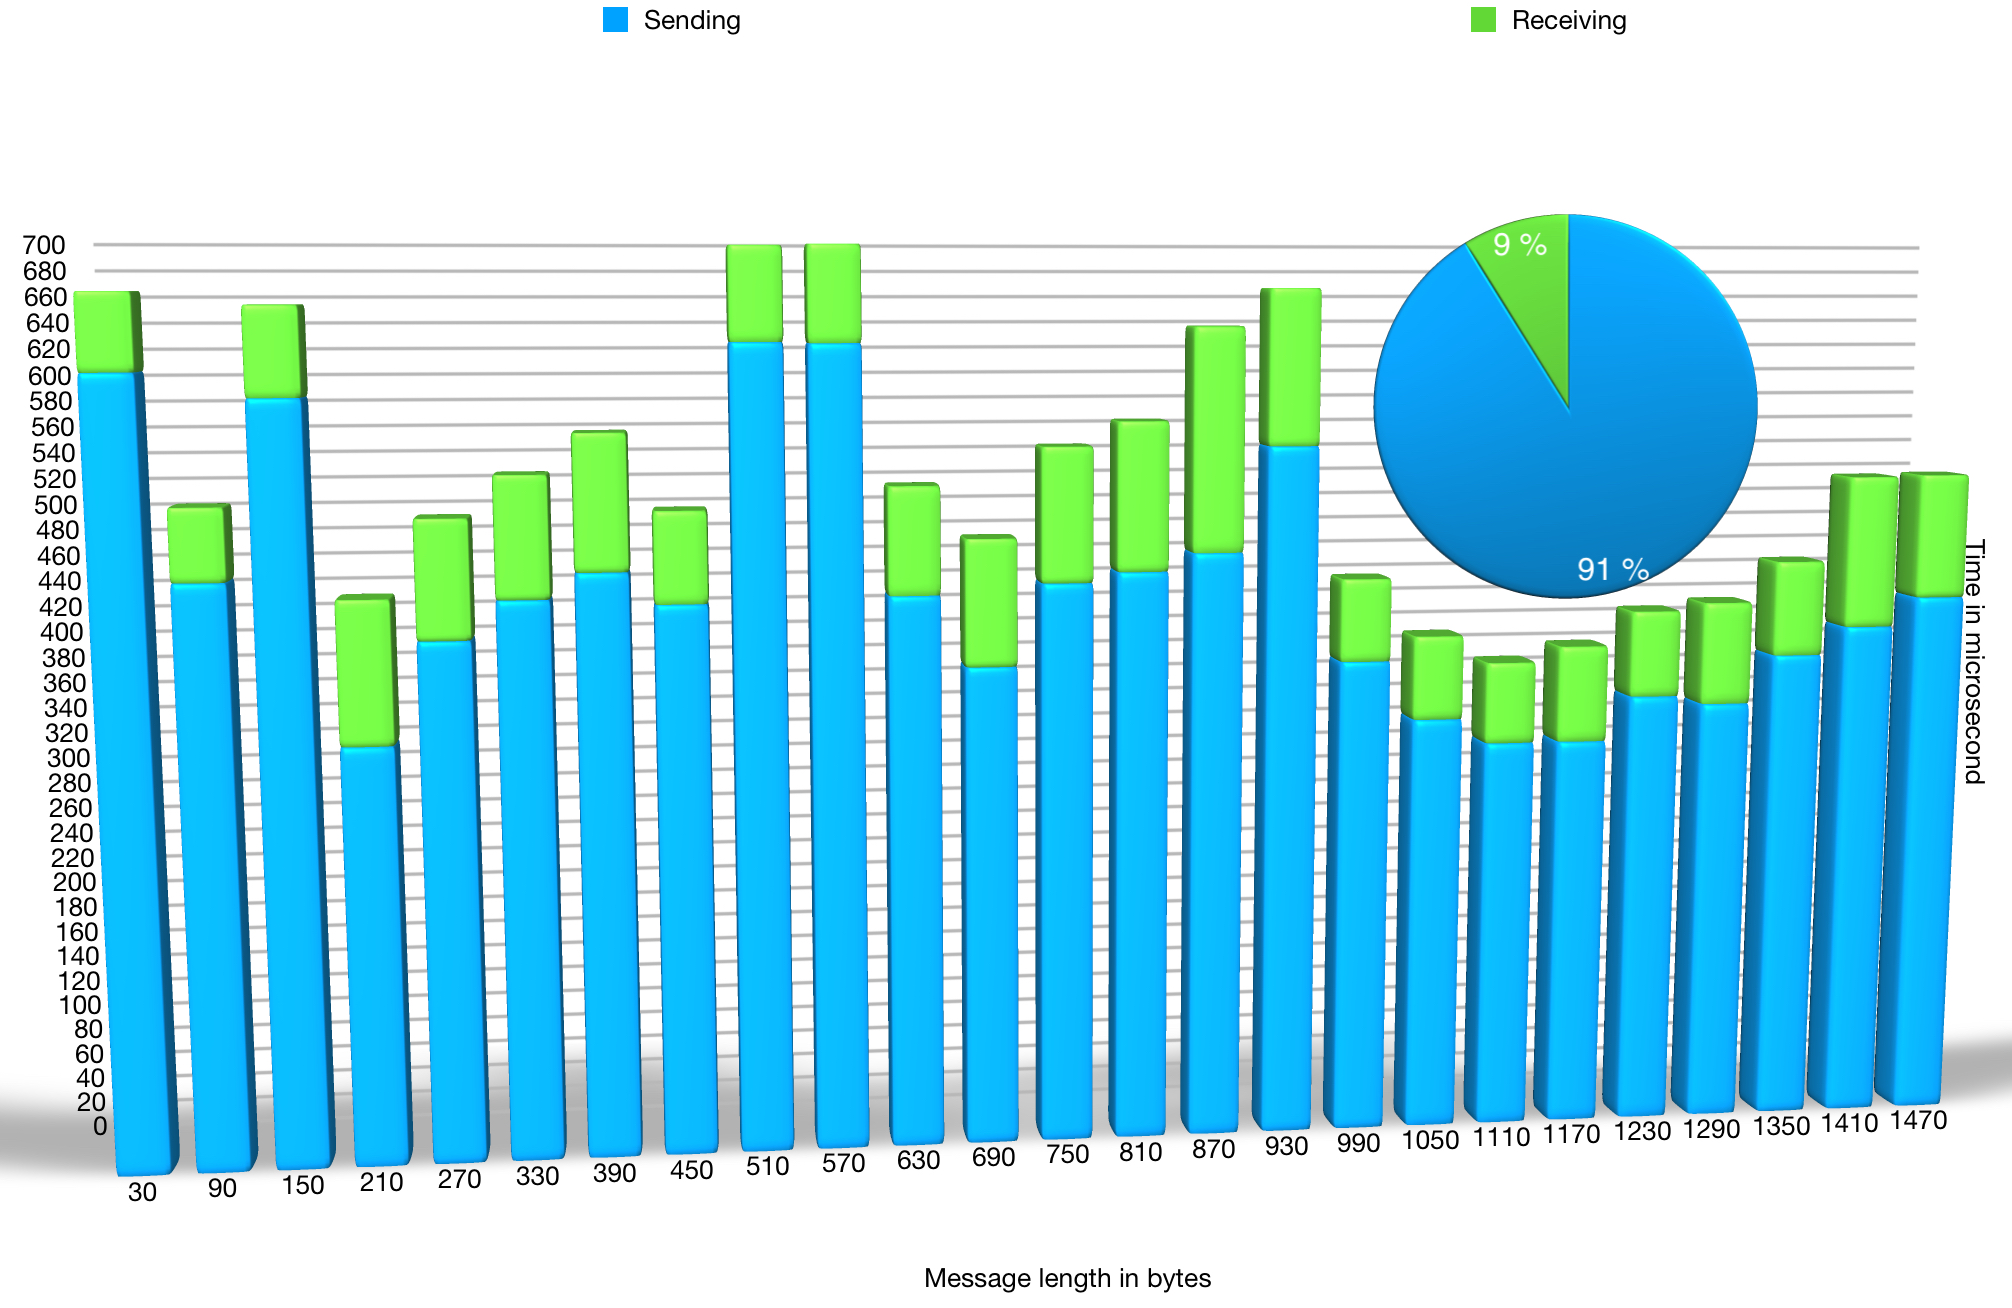
\includegraphics[width=19cm,frame]{figures/realization/original_safetynetp.jpg}
\caption{SafetyNETp before integrating the security layer}\label{original_safetynetp}
\end{figure}


As a second step, we evaluated our security layer.
\autoref{safetynetp_with_scurity_layer} shows the time needed for sending and receiving messages through the
security layer using TLS\_RSA\_WITH\_AES\_128\_CBC\_SHA256 cipher suite. The time includes the encryption, the MAC
calculation and the decryption.

\begin{figure}[H]
\centering
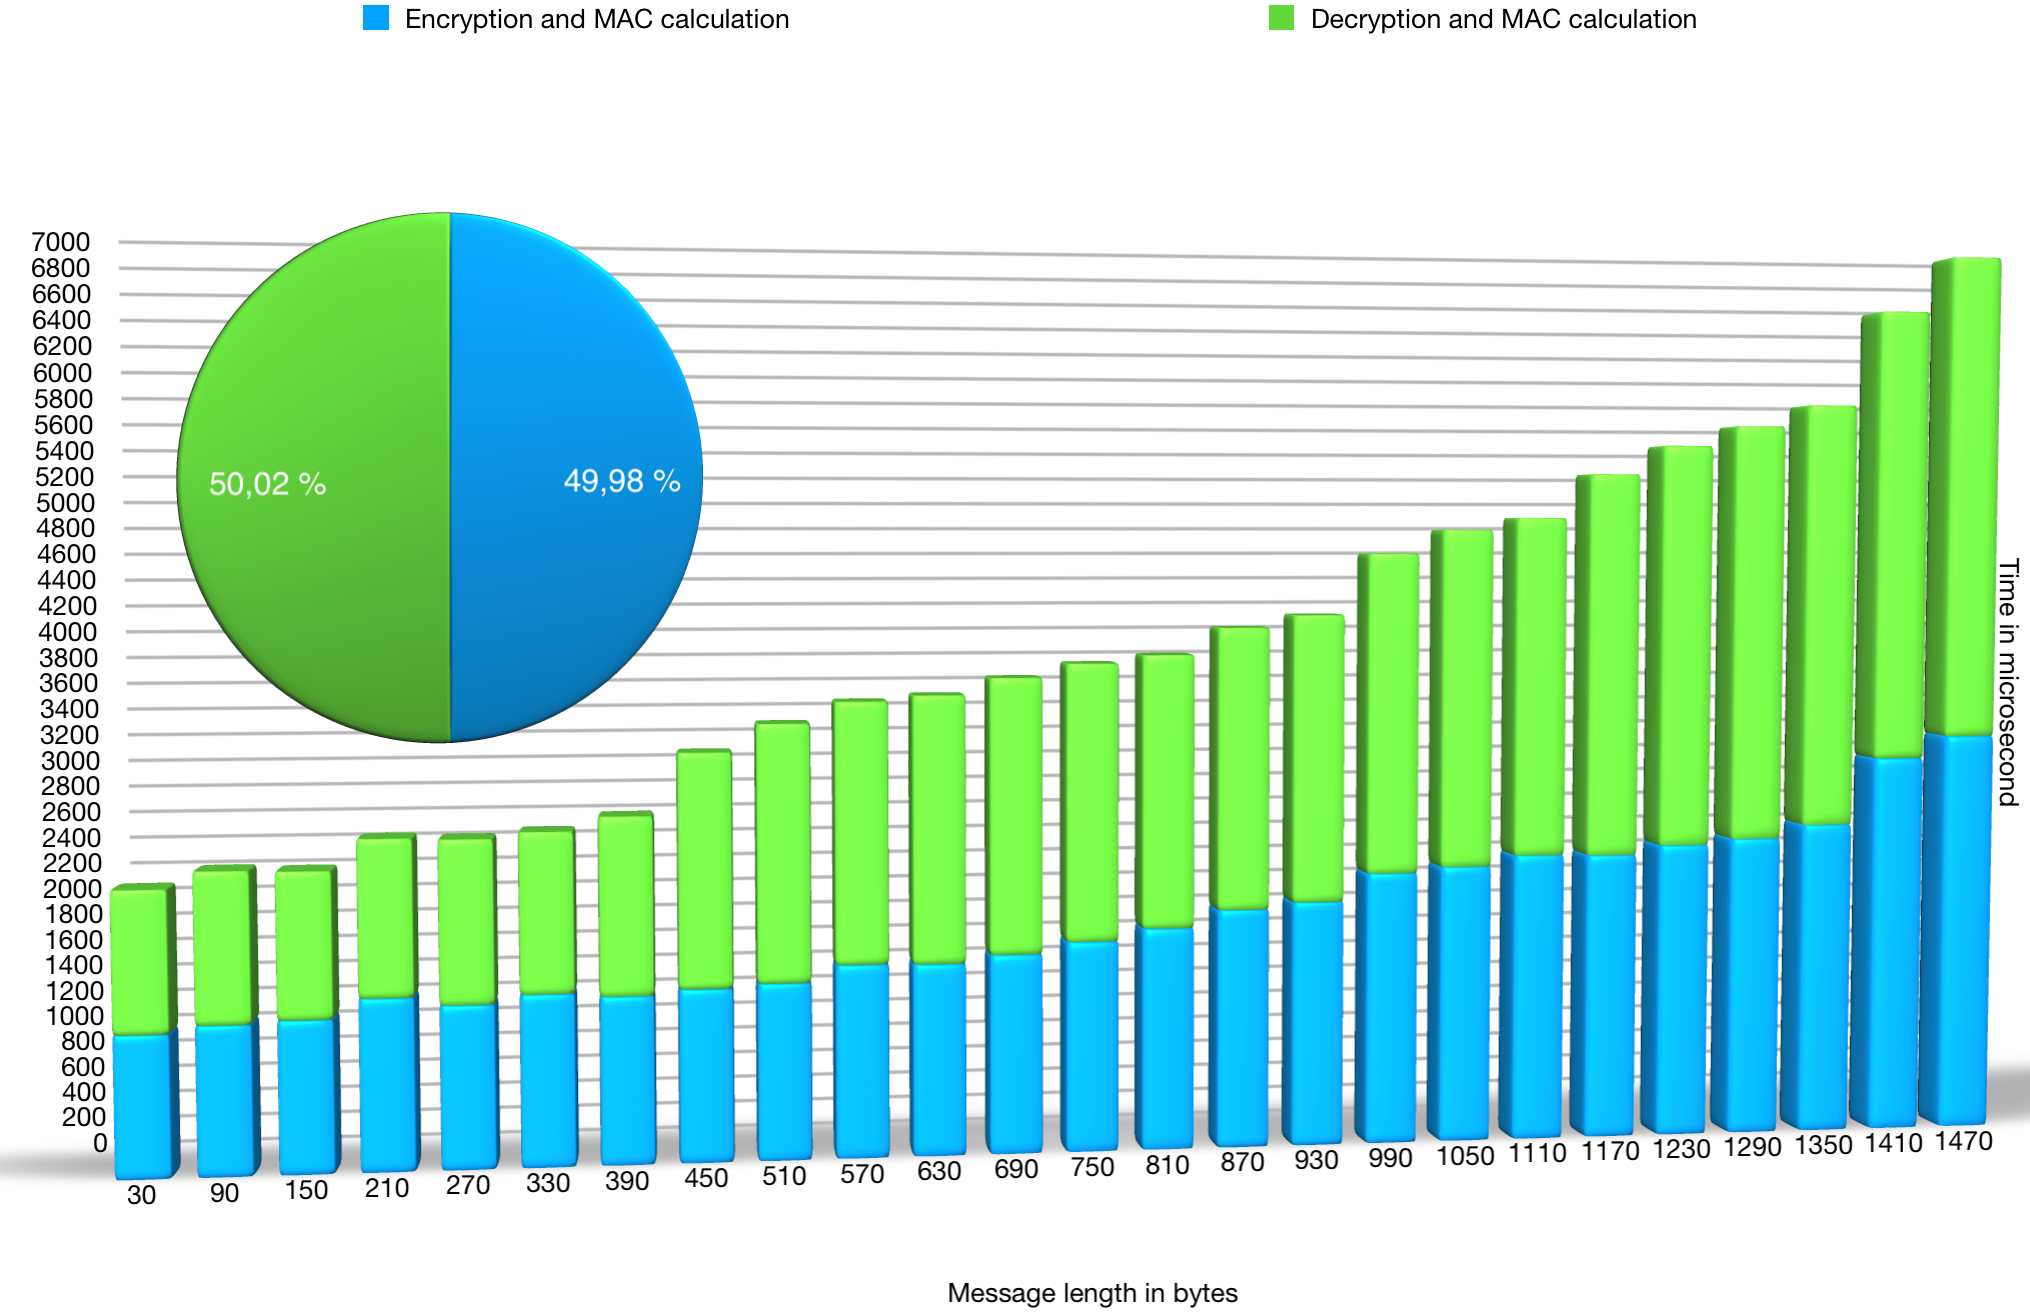
\includegraphics[width=19cm,frame]{figures/realization/safetynetp_with_scurity_layer.jpg}
\caption{SafetyNETp after integrating the security layer}\label{safetynetp_with_scurity_layer}
\end{figure}

The protected messages are encapsulated into DTLS frames then into the security layer frame. This introduces
a data overhead as the secured messages contain the security layer and DTLS headers as well as the MAC.
Furthermore, some encryption algorithms need to add padding to the messages. \autoref{data_overhead} shows the
data overhead.

\begin{figure}[H]
\centering
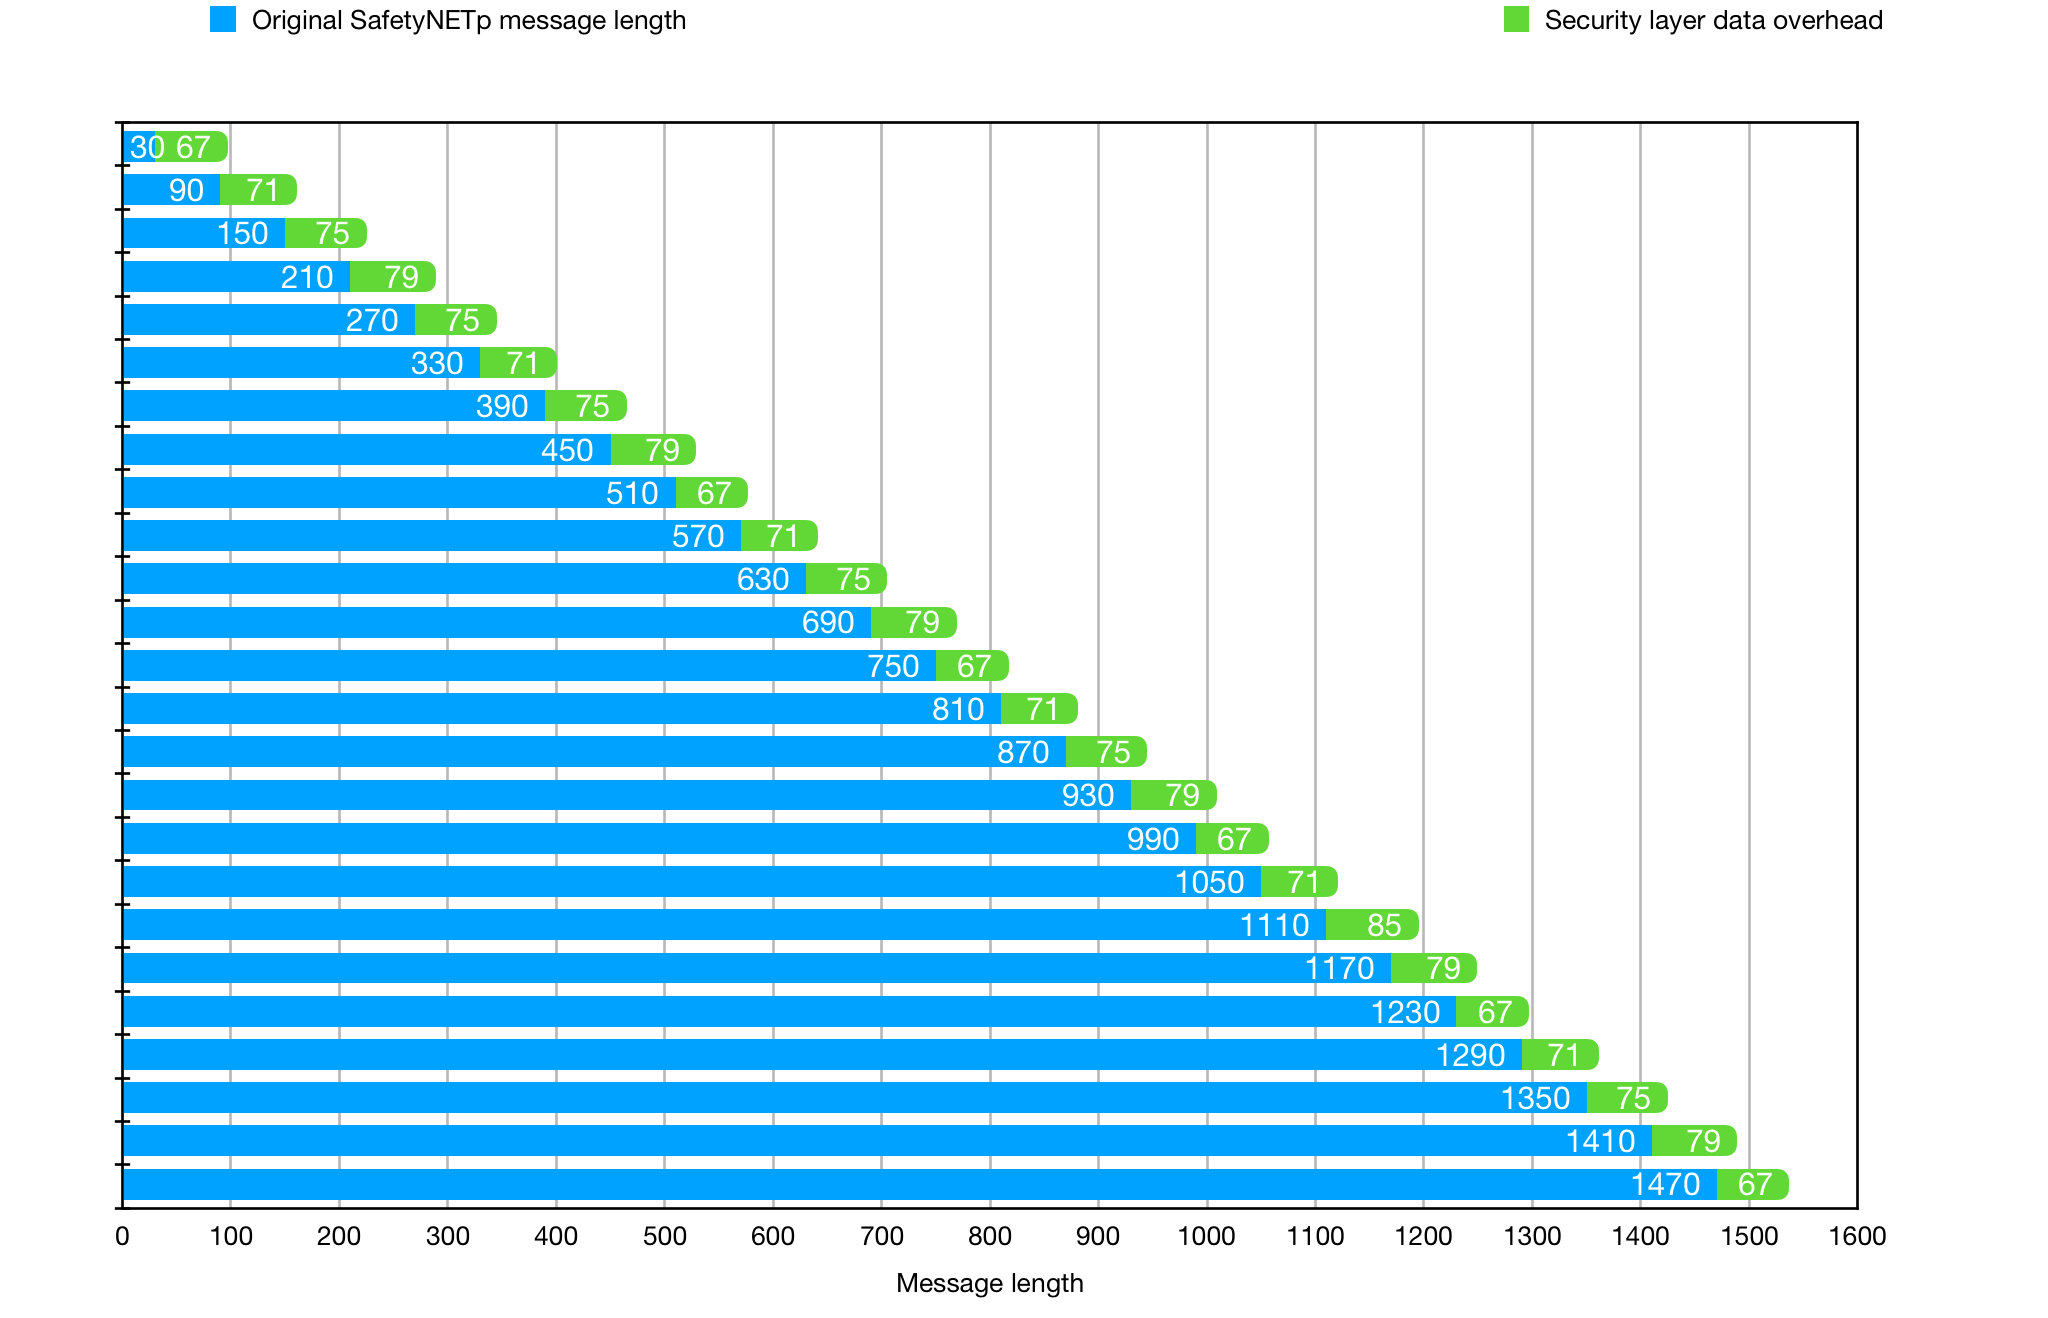
\includegraphics[width=19cm,frame]{figures/realization/data_overhead.jpg}
\caption{Data overhead}\label{data_overhead}
\end{figure}

The startup time of the system without our security layer is equal to the startup time of the SafetyNETp devices
as the devices start exchanging \textit{cyclic data} directly after the startup. However, with our security layer, after the startup,
the devices establish the DTLS handshake before exchanging \textit{cyclic data}. In fact, as shown in \autoref{startup_time_overhead}
the time needed for the devices' startup is equal to \textit{94 seconds}, the time needed to establish the DTLS handshake is equal to
\textit{7 seconds}. Therefore the new startup time is equal to \textit{101 seconds}.


\begin{figure}[H]
\centering
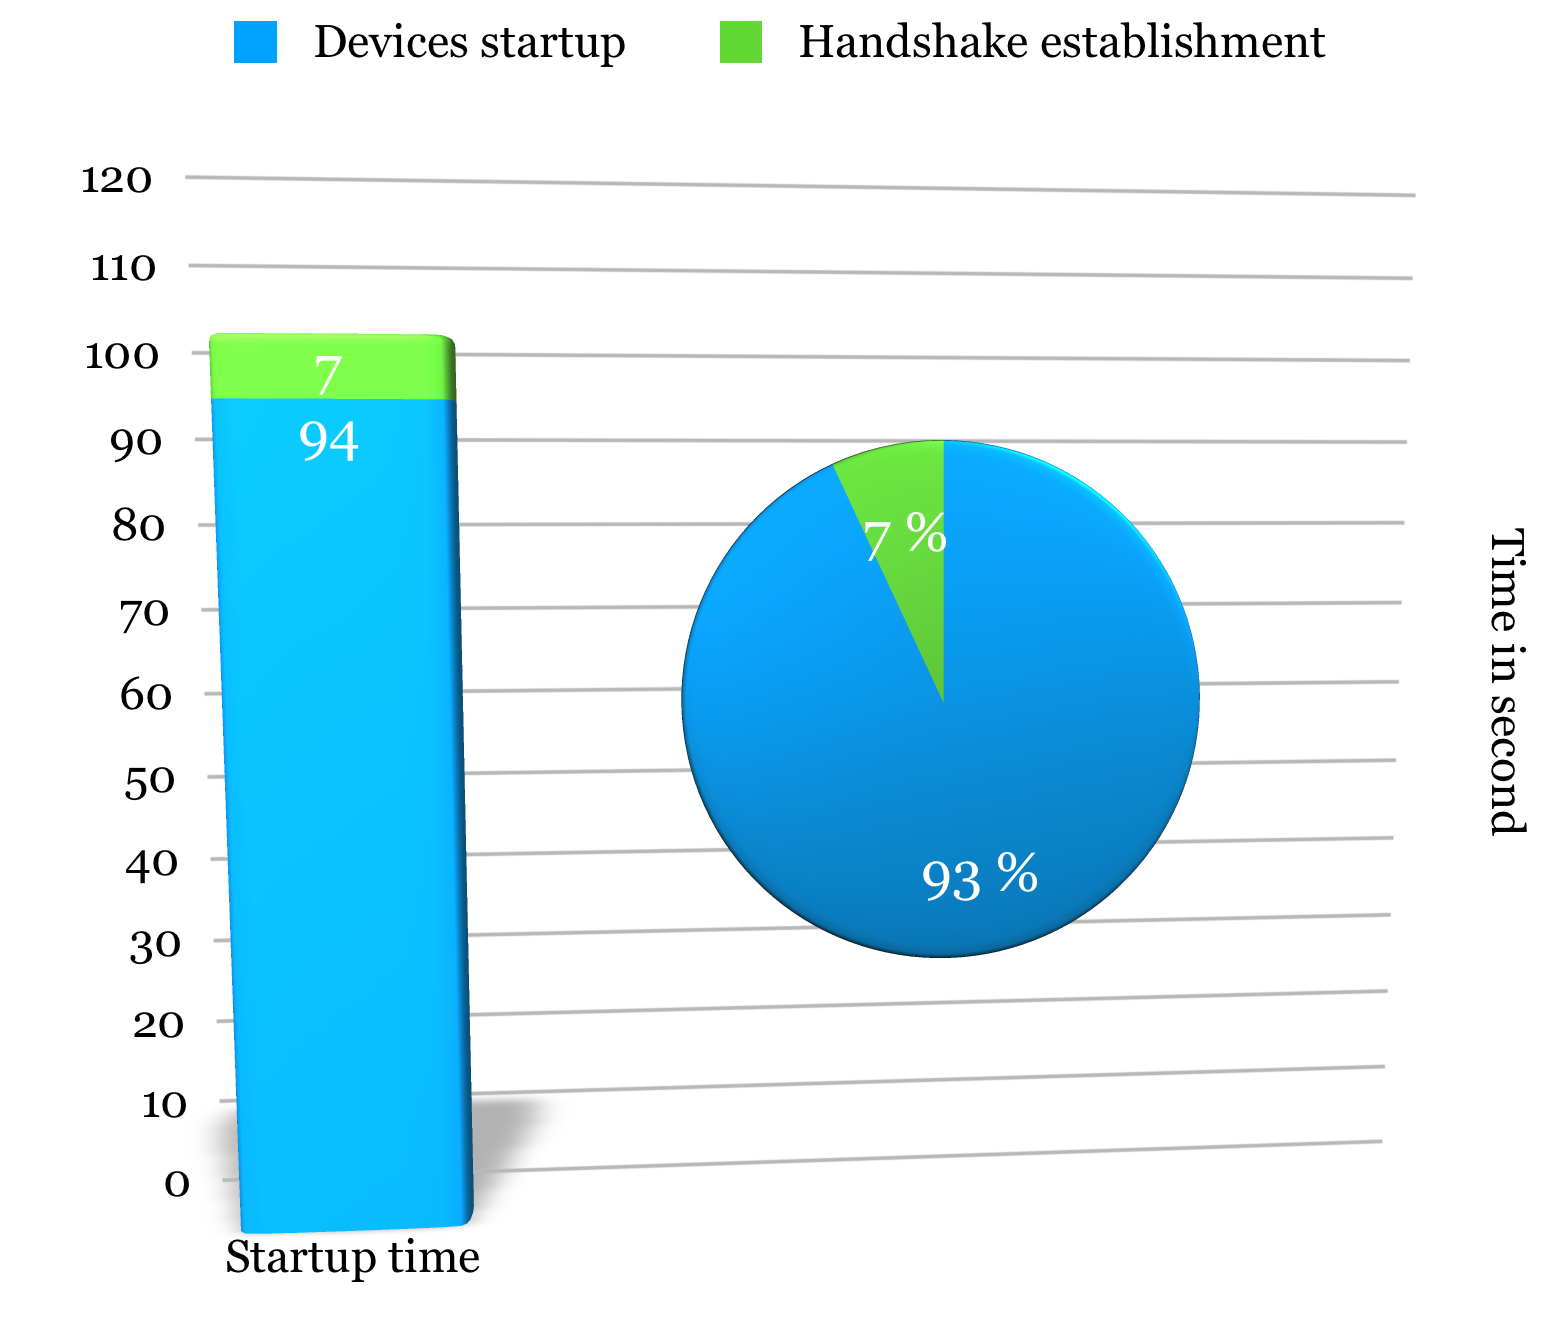
\includegraphics[width=10cm,frame]{figures/realization/startup_time_overhead.jpg}
\caption{Startup time overhead}\label{startup_time_overhead}
\end{figure}


%
% In order to evalute our solution, we performed some perfomance measures by sending 300 messages before
% and after integrating our security layer. In fact, as shown in \autoref{enc_dec_overhead}
% in order to encapsulate the original SafetyNETp message into the security layer frame wich includes
%  encrypting the message, performing
% the MAC calculation, encapsulating the message into DTLS frame and then into the security layer frame,
% the average needed time is \textit{340 microseconds}, the maximum time we have encoutered is \textit{448 microseconds} and the minimun time is \textit{236 microseconds}.
% In order to decapsulate a secured frame wich includes the decryption,the identity and the integrity checks, the average needed
% time is \textit{120 microseconds}, the maximum time is \textit{170 microseconds} and the minimum time is \textit{100 microseconds}.
% As we are using 100 Mbit/second Ethernet, the transmission overhead is insignificant, in fact, it is equal to \textit{2 microseconds}.
% To conclude the maximum total overhead introduced by our security layer is no more than \textit{620 microseconds}.
%
% \begin{figure}[H]
% \centering
% 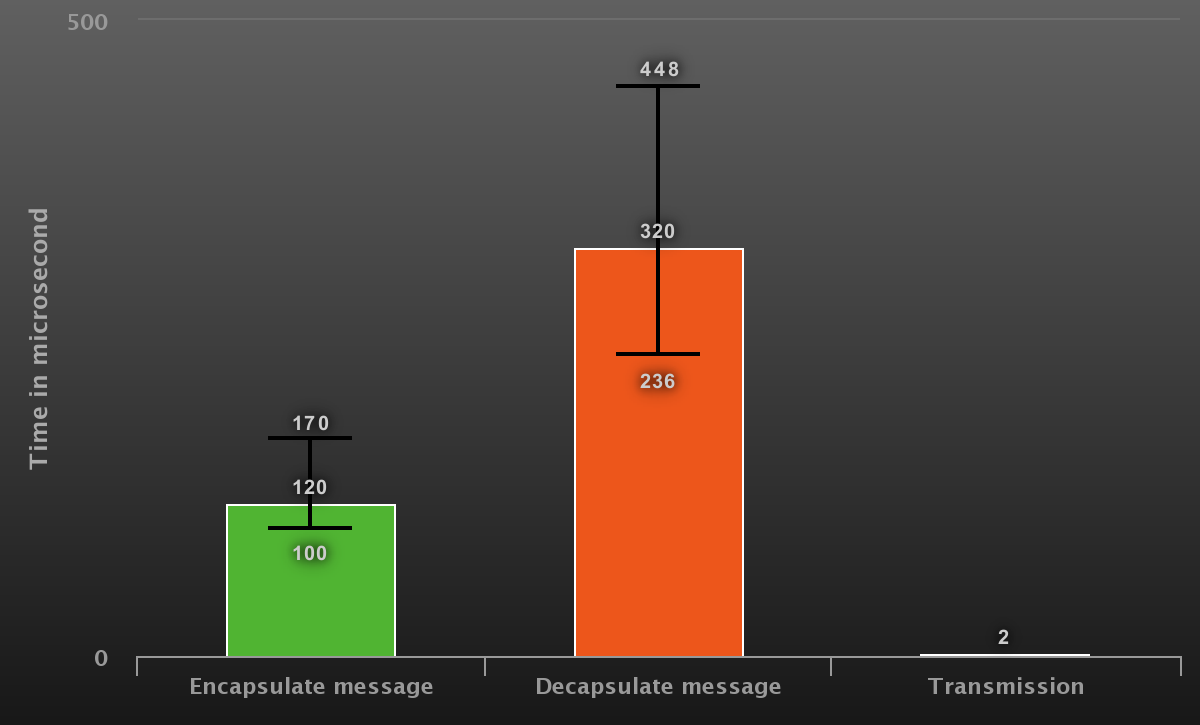
\includegraphics[width=15cm]{figures/realization/enc_dec_overhead.png}
% \caption{Overhead introduced in encapsulating and decapsulating messages}\label{enc_dec_overhead}
% \end{figure}
%
% The startup time of the system without our security layer is equal to the startup time of the SafetyNETp devices
% as the devices start exchanging \textit{cyclic data} directly after the startup. However, with our security layer, after the startup,
% the devices establish the DTLS handshake before exchanging \textit{cyclic data}. In fact, as shown in \autoref{statup_time_overhead}
% the time needed for devices' startup is equal to \textit{94 seconds}, the time needed to estbalish the DTLS handshake is equal to
% \textit{7 seconds}. Therefore the new startup time is equal to \textit{101 seconds}.
%
% \begin{figure}[H]
% \centering
% 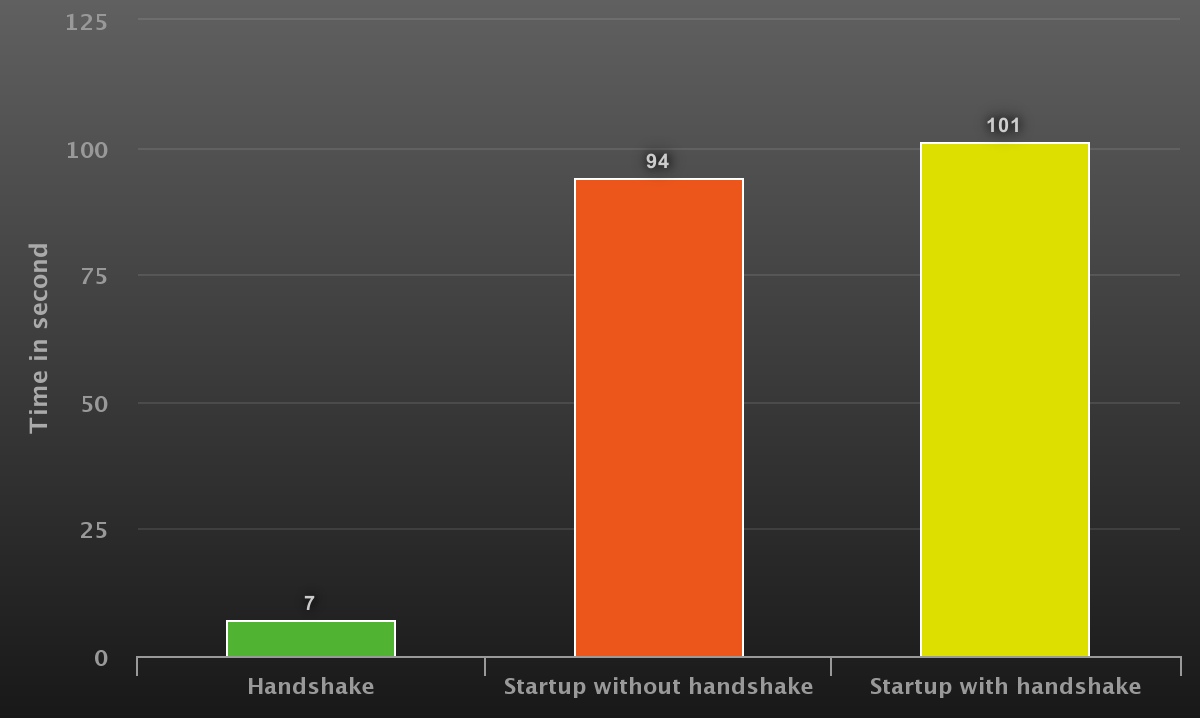
\includegraphics[width=15cm]{figures/realization/statup_time_overhead.png}
% \caption{Startup time overhead}\label{statup_time_overhead}
% \end{figure}
%
% \begin{figure}[H]
% \centering
% \includegraphics[width=19cm]{figures/realization/test.jpeg}
% \caption{Startup time overhead}\label{test}
% \end{figure}

\section*{Conclusion}

 Throughout this chapter, we presented the software and the hardware environments, we outlined the
 important implementation steps and we evaluated finally the performance of our solution.
